% ============================================================================
% Capítulo 5. Diseño
%
% Paquetes que necesita este capítulo en el preámbulo:
%   \usepackage{graphicx}
%   \usepackage{booktabs}
%   \usepackage{amsmath,amssymb,amsthm}
%   \usepackage{algorithm}
%   \usepackage[noend]{algpseudocode}
%   \usepackage{listings}
%   \usepackage{xcolor}
%
%   \newtheorem{proposicion}{Proposición}[chapter]
%   \floatname{algorithm}{Algoritmo}
%   \renewcommand{\listalgorithmname}{Índice de algoritmos}
%   \algrenewcommand\algorithmicwhile{\textbf{mientras}}
%   \algrenewcommand\algorithmicdo{\textbf{hacer}}
%   \algrenewcommand\algorithmicfor{\textbf{para}}
%   \algrenewcommand\algorithmicforall{\textbf{para cada}}
%   \algrenewcommand\algorithmicif{\textbf{si}}
%   \algrenewcommand\algorithmicthen{\textbf{entonces}}
%   \algrenewcommand\algorithmicelse{\textbf{si no}}
%   \algrenewcommand\algorithmicreturn{\textbf{devolver}}
%   \algrenewcommand\algorithmicfunction{\textbf{función}}
%   \algrenewcommand\algorithmicprocedure{\textbf{procedimiento}}
%   \lstdefinestyle{codigo}{basicstyle=\ttfamily\small, columns=fullflexible,
%     frame=lines, breaklines=true, keepspaces=true, showstringspaces=false}
%
% Las figuras están en diagramas/ (fuente .puml y exportación .png).
% Lo que depende del incremento 4 (conexión real con Neo4j) se marca como
% «previsto» y con % TODO: comprobar al implementarlo.
% ============================================================================

\chapter{Diseño}
\label{cap:diseno}

Este capítulo describe el diseño del visor tal como queda al cerrar el incremento~4, en el que el servidor pasa de trabajar con datos simulados a consultar la base de datos Neo4j del proyecto REFRACTS. Se presentan, por este orden, los algoritmos (sección~\ref{sec:algoritmos}), el diseño de los datos (sección~\ref{sec:bd}), las clases (sección~\ref{sec:clases}), la interacción entre ellas en cada operación (sección~\ref{sec:interaccion}) y la organización en paquetes (sección~\ref{sec:paquetes}). Todo lo que se describe corresponde al código del repositorio; las partes que dependen de la conexión con Neo4j y que todavía no están implementadas se señalan como previstas.

% ----------------------------------------------------------------------------
\section{Diseño de algoritmos}
\label{sec:algoritmos}

\subsection{Reparto del cálculo entre servidor y cliente}
\label{sec:reparto}

El reparto del trabajo entre el servidor y el navegador ha cambiado a lo largo de los incrementos, y conviene explicarlo antes de describir cada algoritmo porque condiciona dónde se ejecuta cada uno.

\begin{itemize}
  \item \textbf{Incremento 1.} Todo se ejecutaba en el navegador sobre un fichero de datos de ejemplo. Servía para validar la visualización, pero no es viable con la base de datos real: el navegador no puede descargar el grafo completo.
  \item \textbf{Incremento 2.} El servidor recorría el grafo, calculaba la relevancia de cada nodo, construía el subgrafo y lo enviaba ya terminado. Cada cambio de umbral obligaba a repetir todo el cálculo en el servidor, lo que va en contra de RNF-05 (carga del servidor) cuando hay muchos usuarios.
  \item \textbf{Incrementos 3 y 3b.} El servidor se limita a entregar, en una sola respuesta, el \emph{vecindario} de la entidad: las entidades y relaciones alcanzables por relaciones que superan el umbral. El navegador construye el subgrafo, calcula la centralidad y la disposición. El servidor solo calcula lo que exige acceso a la base de datos: las relaciones derivadas y la relevancia de las relaciones que todavía no la tienen.
  \item \textbf{Incremento 4.} Se mantiene el reparto del incremento 3b; cambia el origen de los datos (Neo4j en lugar de datos simulados) detrás de la misma interfaz \texttt{RepositorioDatos}.
\end{itemize}

La decisión de mover el cálculo al cliente se apoya en dos hechos. Primero, el coste de construir el subgrafo es pequeño frente a la latencia de red (del orden de milisegundos para 150 nodos, sección~\ref{sec:alg-subgrafo}). Segundo, la propiedad de monotonía que se demuestra en la proposición~\ref{prop:vecindario} permite reutilizar un vecindario ya descargado cuando el usuario sube el umbral, de modo que la operación más frecuente (mover el deslizador) no genera peticiones.

La tabla~\ref{tab:notacion} fija la notación que se usa en los análisis de complejidad.

\begin{table}[htbp]
  \centering
  \caption{Notación de los análisis de complejidad.}
  \label{tab:notacion}
  \begin{tabular}{@{}ll@{}}
    \toprule
    Símbolo & Significado \\
    \midrule
    $n$ & entidades del vecindario (como mucho \texttt{maxEntidadesVecindario} $=2000$) \\
    $m$ & relaciones derivadas del vecindario \\
    $k$ & nodos del subgrafo (como mucho \texttt{maxNodos} $=150$) \\
    $m_k$ & relaciones del subgrafo \\
    $P$ & tamaño de la lista de candidatos pendientes \\
    $p$ & entidades unidas a un mismo intermediario \\
    $h$ & profundidad de la jerarquía de tipos (\texttt{IS\_A}) \\
    $N$ & entradas del índice de nombres; $L$ longitud de un nombre \\
    \bottomrule
  \end{tabular}
\end{table}

\subsection{Recorrido del vecindario en el servidor}
\label{sec:alg-vecindario}

\paragraph{Propósito.} Entregar al navegador, en una sola petición, todo lo necesario para construir el subgrafo de una entidad con un umbral dado (RF-08 a RF-13), sin enviar el grafo completo (RNF-05). Lo implementa \texttt{RepositorioDatos.obtener\_vecindario}; en el incremento~4, \texttt{RepositorioNeo4j}.

\paragraph{Algoritmo.} Es un recorrido en anchura desde la entidad central que solo atraviesa relaciones derivadas cuya relevancia supera el umbral (algoritmo~\ref{alg:vecindario}). La relevancia de cada relación se obtiene de forma perezosa: se lee de la base de datos y, si falta, se calcula y se guarda (sección~\ref{sec:alg-asignacion}). Un mismo intermediario produce varias relaciones derivadas y su relevancia se pide una sola vez por petición.

\begin{algorithm}[htbp]
  \caption{Recorrido del vecindario (\texttt{obtener\_vecindario}).}
  \label{alg:vecindario}
  \begin{algorithmic}[1]
    \Function{ObtenerVecindario}{$e_0$, $u$, $maxEntidades$}
      \State $encontrados \gets \{e_0\}$; $cola \gets [e_0]$; $relaciones \gets \emptyset$; $valores \gets \emptyset$
      \State $recortado \gets \textbf{falso}$
      \While{$cola$ no vacía}
        \State $e \gets$ sacar el primero de $cola$
        \ForAll{$r \in$ \Call{RelacionesDe}{$e$}} \Comment{regla genérica, alg.~\ref{alg:derivadas}}
          \If{$r.idIntermedio \notin valores$}
            \State $valores[r.idIntermedio] \gets$ \Call{ObtenerRelevancia}{$r.idIntermedio$, $r.tipo$}
          \EndIf
          \State $v \gets valores[r.idIntermedio]$
          \If{$v > u$}
            \State añadir $r$ (con $valor = v$) a $relaciones$
            \State $o \gets$ el otro extremo de $r$
            \If{$o \notin encontrados$}
              \If{$|encontrados| < maxEntidades$}
                \State añadir $o$ a $encontrados$ y al final de $cola$
              \Else
                \State $recortado \gets \textbf{verdadero}$
              \EndIf
            \EndIf
          \EndIf
        \EndFor
      \EndWhile
      \State \Return $(encontrados$, relaciones entre $encontrados$, $recortado)$
    \EndFunction
  \end{algorithmic}
\end{algorithm}

\paragraph{Corrección.} La propiedad que justifica que el vecindario basta es la siguiente.

\begin{proposicion}
\label{prop:vecindario}
Sea la relevancia de un nodo $x$ el máximo, sobre los caminos $e_0=x_0,x_1,\dots,x_l=x$, del producto $\prod_{i=1}^{l} r_i$, donde $r_i\in[0,1]$ es la relevancia de la relación entre $x_{i-1}$ y $x_i$. Si la relevancia de $x$ supera el umbral $u$, todas las relaciones del camino que la alcanza superan $u$.
\end{proposicion}

\begin{proof}
Para cualquier $j$, $\prod_{i=1}^{l} r_i = r_j\cdot\prod_{i\neq j} r_i \le r_j$, porque el segundo factor está en $[0,1]$. Si el producto es mayor que $u$, entonces $r_j > u$ para todo $j$. Por tanto el camino solo usa relaciones que el recorrido atraviesa, y $x$ y todo su camino están en el vecindario.
\end{proof}

Dos consecuencias se usan en el diseño. El vecindario puede contener nodos de más (por ejemplo, uno a $0{,}5\cdot0{,}5=0{,}25$ con $u=0{,}3$), que el navegador descarta al construir el subgrafo. Y un vecindario calculado con umbral $u$ sirve para cualquier $u'\ge u$, lo que permite la reutilización descrita en la sección~\ref{sec:alg-subgrafo}.

\paragraph{Complejidad.} Cada entidad entra una vez en la cola y cada relación derivada se examina desde sus dos extremos: $O(n+m)$ operaciones en memoria. Con Neo4j el coste dominante es el número de consultas. Si se hace una consulta por entidad, son $n$ viajes de ida y vuelta; el diseño previsto agrupa la frontera de cada nivel en una sola consulta con \texttt{UNWIND} (listado~\ref{lst:cypher-vecindario}), con lo que el número de consultas pasa a ser la profundidad del recorrido. % TODO: medir con la BD real.

\paragraph{Parámetros.} Umbral $u$: el de la petición, redondeado hacia abajo a dos decimales (\texttt{redondear\_hacia\_abajo}) para que peticiones casi iguales compartan caché; el redondeo es hacia abajo para que el vecindario resultante siga conteniendo el pedido. \texttt{maxEntidadesVecindario} $=2000$, fijado en el servidor y no modificable desde la petición (RNF-13); si se alcanza, la respuesta lleva \texttt{recortado = true}.

\paragraph{Alternativas descartadas.}
\begin{itemize}
  \item \emph{Recorrido en profundidad.} Con el tope de entidades, la anchura garantiza que, si hay que recortar, se pierden las entidades más alejadas en número de saltos; la profundidad podría agotar el tope en una sola rama.
  \item \emph{Construir el subgrafo en el servidor} (incremento 2). Descartado por RNF-05, como se explica en la sección~\ref{sec:reparto}.
  \item \emph{Recorrido con caminos de longitud variable de Cypher} (\texttt{[*1..d]}). Necesita conocer la relevancia antes de recorrer, pero esta se asigna durante el recorrido. Además, el número de caminos crece de forma exponencial con $d$.
\end{itemize}

\subsection{Regla genérica de relaciones derivadas}
\label{sec:alg-derivadas}

\paragraph{Propósito.} En REFRACTS las entidades no se relacionan entre sí directamente, sino a través de nodos intermediarios (\texttt{Relationship}, \texttt{Event} y sus subtipos). El visor necesita aristas entre entidades (RF-08), así que el servidor las deriva. La regla no contiene nombres de etiquetas en el código: la clasificación de cada etiqueta (entidad, auxiliar o intermediario) se lee de la configuración (RNF-16), y todo lo que no es entidad ni auxiliar se trata como intermediario. Lo implementan \texttt{ProyectorRelaciones} y \texttt{ClasificadorEtiquetas}.

\begin{algorithm}[htbp]
  \caption{Relaciones derivadas de una entidad (\texttt{relaciones\_de}).}
  \label{alg:derivadas}
  \begin{algorithmic}[1]
    \Function{RelacionesDe}{$e$}
      \State $R \gets \emptyset$
      \ForAll{enlace $(e, x)$ de tipo no incluido en \texttt{relacionesIgnoradas}}
        \If{$x$ es una entidad} \Comment{regla 2: relación directa}
          \State añadir a $R$ la relación $(e, x)$ con el tipo del enlace
        \ElsIf{$x$ es intermediario \textbf{y} no es de \texttt{tiposSinRelacion}}
          \State $Q \gets$ entidades unidas a $x$ por enlaces no ignorados
          \If{$2 \le |Q| \le$ \texttt{maxParticipantesIntermediario}} \Comment{regla 1}
            \State $t \gets$ etiqueta más específica de $x$
            \ForAll{$q \in Q$, $q \neq e$}
              \State añadir a $R$ la relación $(e, q)$ de tipo $t$, con roles, periodo, lugar y fecha de $x$
            \EndFor
          \EndIf
        \EndIf
      \EndFor
      \State \Return $R$
    \EndFunction
  \end{algorithmic}
\end{algorithm}

Cada relación derivada tiene como identificador \texttt{idIntermedio|idA|idB}, con la pareja ordenada por identificador, de modo que se obtiene la misma relación desde cualquiera de sus dos extremos. Dos relaciones con la misma pareja y distinto intermediario son distintas (RF-38).

\paragraph{Complejidad y límite.} Un intermediario con $p$ participantes produce $p(p-1)/2$ relaciones: el coste es cuadrático en $p$. Un evento con 50 asistentes daría 1225 aristas que no aportan información sobre relaciones personales y saturarían el subgrafo. Por eso se ignoran los intermediarios con más de \texttt{maxParticipantesIntermediario} $=10$ participantes, lo que acota a 45 las relaciones por intermediario. Los tipos \texttt{Birth}, \texttt{Death} y \texttt{Live} (\texttt{tiposSinRelacion}) describen a una sola persona; no generan relaciones y se muestran en el detalle de la entidad.

\paragraph{Alternativa descartada.} Escribir una consulta o una función por cada combinación de etiquetas (persona–persona por \texttt{Relationship}, persona–obra por \texttt{Creation}, etc.). Obligaría a modificar el código cada vez que el modelo de REFRACTS añada un tipo, lo que contradice el principio abierto/cerrado y RNF-16.

\subsection{Relevancia por tipo con herencia}
\label{sec:alg-tipo}

\paragraph{Propósito.} Las relaciones de REFRACTS no tienen un valor de relevancia. Hay que asignarles uno que refleje lo estrecha que es la relación (un matrimonio más que una exposición compartida). La estrategia \texttt{RelevanciaPorTipo} asigna un peso según el tipo y, si el tipo no tiene peso, usa el de su antecesor más cercano en la jerarquía \texttt{IS\_A} (algoritmo~\ref{alg:tipo}). Así un tipo nuevo, como un hipotético \texttt{Apprenticeship} bajo \texttt{Professional}, recibe un peso razonable sin tocar la configuración.

\begin{algorithm}[htbp]
  \caption{Relevancia de un tipo (\texttt{RelevanciaPorTipo.calcular\_relevancia}).}
  \label{alg:tipo}
  \begin{algorithmic}[1]
    \Function{CalcularRelevancia}{$t$}
      \If{$t \in pesos$} \State \Return $pesos[t]$ \EndIf
      \ForAll{$a \in$ \Call{Padres}{$t$}} \Comment{del más cercano al más lejano}
        \If{$a \in pesos$} \State \Return $pesos[a]$ \EndIf
      \EndFor
      \State \Return \texttt{pesoPorDefecto} \Comment{0,5}
    \EndFunction
  \end{algorithmic}
\end{algorithm}

El coste es $O(h)$. La tabla~\ref{tab:pesos} recoge los pesos iniciales.

\begin{table}[htbp]
  \centering
  \caption{Pesos iniciales de \texttt{RelevanciaPorTipo} (\texttt{versionPesos} $=1$). Pendientes de validar con el tutor.}
  \label{tab:pesos}
  \begin{tabular}{@{}lr@{\hspace{2.5em}}lr@{}}
    \toprule
    Tipo de relación & Peso & Tipo de evento & Peso \\
    \midrule
    \texttt{Marriage} (matrimonio) & 0,95 & \texttt{Creation} (creación) & 0,90 \\
    \texttt{Filiation} (filiación) & 0,90 & \texttt{Fund} (fundación) & 0,85 \\
    \texttt{Mentorship} (mentoría) & 0,85 & \texttt{Work} (trabajo) & 0,60 \\
    \texttt{Friendship} (amistad) & 0,75 & \texttt{Wedding} (boda) & 0,60 \\
    \texttt{Related} (parentesco) & 0,70 & \texttt{Exposition} (exposición) & 0,50 \\
    \texttt{coworking} (colaboración) & 0,65 & \texttt{Event} (otros) & 0,40 \\
    \texttt{Employement} (empleo) & 0,60 & & \\
    \texttt{Professional} & 0,55 & & \\
    \texttt{Relationship} (genérica) & 0,50 & \texttt{pesoPorDefecto} & 0,50 \\
    \bottomrule
  \end{tabular}
\end{table}

% TODO: validar los pesos con el tutor y, si cambian, subir versionPesos.

\paragraph{Alternativas descartadas.} Calcular la relevancia a partir de la estructura del grafo (por ejemplo, el número de eventos compartidos entre dos personas) exigiría recorrer zonas del grafo que no se van a mostrar y no tiene en cuenta el significado del vínculo. Pedir a los expertos un valor para cada relación no es viable con miles de intermediarios. El peso por tipo es una primera aproximación que se puede sustituir: \texttt{EstrategiaRelevancia} es una interfaz, y otra estrategia se conecta sin cambiar \texttt{AsignadorRelevancia} (patrón Estrategia, sección~\ref{sec:patrones}).

\subsection{Asignación perezosa de la relevancia}
\label{sec:alg-asignacion}

\texttt{AsignadorRelevancia.obtener} decide si una relevancia guardada vale o hay que calcularla (algoritmo~\ref{alg:asignacion}). Cada valor guardado lleva su origen (\texttt{relevanceSource}: \texttt{auto} o \texttt{manual}) y la versión de la tabla de pesos con la que se calculó (\texttt{relevanceVersion}).

\begin{algorithm}[htbp]
  \caption{Obtención de la relevancia de un intermediario (\texttt{AsignadorRelevancia.obtener}).}
  \label{alg:asignacion}
  \begin{algorithmic}[1]
    \Function{ObtenerRelevancia}{$id$, $t$}
      \State $g \gets$ \Call{Leer}{$id$} \Comment{\texttt{AlmacenRelevancias}}
      \If{$g \neq \textbf{nulo}$ \textbf{y} ($g.origen = \texttt{manual}$ \textbf{o} $g.version = \texttt{versionPesos}$)}
        \State $reutilizadas \gets reutilizadas + 1$
        \State \Return $g.valor$
      \EndIf
      \State $v \gets estrategia.$\Call{CalcularRelevancia}{$t$}
      \State \Call{Guardar}{$id$, $v$, \texttt{versionPesos}}
      \State $asignadas \gets asignadas + 1$
      \State \Return $v$
    \EndFunction
  \end{algorithmic}
\end{algorithm}

Con este esquema solo se calcula la relevancia de las relaciones que algún usuario llega a recorrer, y cada una una sola vez por versión de los pesos. Un valor manual (por ejemplo, corregido por un experto) nunca se sobrescribe. Los contadores \texttt{asignadas} y \texttt{reutilizadas} se devuelven en cada vecindario y se muestran en la barra de rendimiento, lo que permite comprobar en uso real que las relevancias se reutilizan.

La alternativa sería un proceso por lotes que asignase la relevancia a toda la base de datos de una vez. Se descartó porque obliga a recalcular todo cada vez que cambian los pesos o el modelo, y escribe en zonas que quizá nadie consulte.

\subsection{Construcción del subgrafo «primero el mejor»}
\label{sec:alg-subgrafo}

\paragraph{Propósito.} Seleccionar el entorno relevante de la entidad central: los nodos cuya relevancia supera el umbral, como mucho \texttt{maxNodos}, y quedándose con los más relevantes si hay más (RF-08 a RF-12). La relevancia de un nodo es el producto de las relevancias de las relaciones de su mejor camino desde la central, que vale~1. Lo implementa \texttt{ConstructorSubgrafo.construir} con la estrategia \texttt{RelevanciaDesdeBD}, que lee el valor asignado por el servidor y lo acota a $[0,1]$.

\begin{algorithm}[htbp]
  \caption{Construcción del subgrafo (\texttt{ConstructorSubgrafo.construir}).}
  \label{alg:subgrafo}
  \begin{algorithmic}[1]
    \Function{Construir}{$e_0$, $u$, $maxNodos$}
      \State $S \gets$ subgrafo con $e_0$ (relevancia 1, nivel 0)
      \State $pendientes \gets$ \Call{Expandir}{$e_0$, $S$, $u$}
      \While{$pendientes$ no vacía \textbf{y} $|S| < maxNodos$}
        \State $c \gets$ el candidato de mayor relevancia de $pendientes$ (se quita)
        \If{$c \notin S$} \Comment{las copias peores se descartan aquí}
          \State añadir $c$ a $S$
          \State añadir \Call{Expandir}{$c$, $S$, $u$} a $pendientes$
        \EndIf
      \EndWhile
      \State calcular la centralidad de cada nodo de $S$ \Comment{sección~\ref{sec:alg-centralidad}}
      \State \Return $S$
    \EndFunction
    \Statex
    \Function{Expandir}{$x$, $S$, $u$}
      \State $mejor \gets \emptyset$ \Comment{mejor relación hacia cada vecino}
      \ForAll{relación $r$ de $x$ con relevancia $r.rel > u$}
        \State $y \gets$ el otro extremo de $r$
        \If{$y \in S$} \State añadir $r$ a $S$ \Comment{se guardan todas las del par (RF-38)}
        \ElsIf{$y \notin mejor$ \textbf{o} $r.rel > mejor[y].rel$} \State $mejor[y] \gets r$
        \EndIf
      \EndFor
      \State \Return $\{\, (y,\ x.rel \cdot mejor[y].rel,\ x.nivel+1) : x.rel \cdot mejor[y].rel > u \,\}$
    \EndFunction
  \end{algorithmic}
\end{algorithm}

\paragraph{Relación con Dijkstra.} Maximizar un producto de valores en $(0,1]$ equivale a minimizar la suma de sus logaritmos cambiados de signo, $\sum -\log r_i$, que son pesos no negativos. El algoritmo~\ref{alg:subgrafo} es, por tanto, el algoritmo de Dijkstra sobre esos pesos, con dos cortes: se detiene al llegar a \texttt{maxNodos} y no expande caminos cuyo producto no supera el umbral. De ahí se sigue la misma propiedad que en Dijkstra: cuando un nodo sale de la lista de pendientes, su relevancia es ya la mejor posible, porque cualquier otro camino pasa por un candidato pendiente de relevancia menor o igual y, por la proposición~\ref{prop:vecindario}, no puede mejorarla. Como consecuencia, los nodos entran en orden decreciente de relevancia y, al cortar en \texttt{maxNodos}, quedan exactamente los más relevantes. \cite{TODO}

\paragraph{Complejidad.} En la implementación actual la lista de pendientes es un vector y la extracción del máximo lo recorre entero (\texttt{\#sacarElMasRelevante}), con coste $O(P)$. El coste total es $O(k\cdot P + m_k)$, con $P$ acotado por el número de relaciones examinadas. Con $k\le150$ y vecindarios de unos cientos de relaciones el cálculo tarda unos 15~ms la primera vez y pocos milisegundos al cambiar el umbral (medido en el navegador con los datos simulados). Una cola de prioridad con montículo binario daría $O((k+m)\log m)$; se deja como mejora si los vecindarios reales resultan mucho mayores. % TODO: revisar con los tiempos medidos sobre Neo4j.

\paragraph{Por qué no una búsqueda por niveles.} Un recorrido en anchura limitado a una profundidad fija (por ejemplo, dos saltos) trata igual un vecino unido por un matrimonio que uno unido por una exposición, y su tamaño depende mucho de la entidad: dos saltos desde una persona muy conectada pueden ser miles de nodos, y desde una poco conectada, muy pocos. El criterio de relevancia acumulada se adapta a cada entidad y respeta el significado de los vínculos.

\paragraph{Reutilización del vecindario.} \texttt{GestorSubgrafos} guarda el último vecindario recibido y su umbral $u_g$. Una petición de la misma entidad con umbral $u\ge u_g$ no va al servidor: por la proposición~\ref{prop:vecindario}, todo camino que supera $u$ supera $u_g$ y está en el vecindario guardado. Con $u<u_g$ podrían faltar relaciones de valor entre $u$ y $u_g$, y se pide un vecindario nuevo. El navegador guarda el umbral que devuelve la respuesta (ya redondeado hacia abajo), no el pedido.

\paragraph{Varias relaciones entre el mismo par (RF-38).} Para decidir si un vecino entra y con qué relevancia se usa la mejor relación hacia él; una vez dentro, se añaden todas las relaciones que lo unen con nodos del subgrafo. \texttt{EnlaceVisual} dibuja las relaciones de un mismo par como curvas de Bézier cuadráticas separadas 1,6 unidades a cada lado de la recta, para que se distingan.

\paragraph{Parámetros.} Umbral: 0,3 por defecto (\texttt{umbralPorDefecto}), modificable con el deslizador entre 0,05 y 1 en pasos de 0,05. \texttt{maxNodos} $=150$. Ambos vienen de \texttt{/api/configuracion}.

\subsection{Ajuste del umbral inicial}
\label{sec:alg-ajuste}

Con un umbral fijo, el tamaño del subgrafo varía mucho de una entidad a otra: con 0,3, casi todas las entidades de los datos de prueba llegaban al tope de 150 nodos. Para que cada entidad se abra con un grafo de tamaño parecido, \texttt{AjustadorUmbral} elige el umbral inicial de cada entidad de forma que salgan aproximadamente \texttt{nodosObjetivo} nodos (100 por defecto).

El cálculo aprovecha que, por la proposición~\ref{prop:vecindario}, con umbral $u$ entran la central y los nodos de relevancia mayor que $u$, sin pasar de \texttt{maxNodos}. \texttt{GestorSubgrafos.obtenerSubgrafoAjustado} construye una vez el subgrafo sin tope sobre el vecindario, obtiene la relevancia de cada nodo, cuenta cuántos nodos saldrían con cada uno de los 20 valores del deslizador y se queda con el más cercano al objetivo; en caso de empate, con el umbral más alto. Si con todo el vecindario pedido con el umbral de la configuración no se alcanza el objetivo, se pide otro con el umbral mínimo (0,05). El coste es el de una construcción sin tope más $O(20\cdot n)$. El ajuste solo se aplica al abrir una entidad; si el usuario mueve el deslizador, se respeta su valor.

\subsection{Centralidad de grado ponderada}
\label{sec:alg-centralidad}

El tamaño de cada nodo representa lo conectado que está dentro del subgrafo (RF-37). \texttt{CalculadorCentralidad} usa la centralidad de grado ponderada, normalizada por el máximo:
\begin{equation}
  C(x) = \frac{\sum_{r \ni x} r.rel}{\max_{y} \sum_{r \ni y} r.rel},
\end{equation}
donde las sumas recorren las relaciones del subgrafo; si el máximo es 0, todos los nodos valen 0. El coste es $O(k + m_k)$. El radio del nodo es $0{,}45 + 1{,}35\sqrt{C(x)}$ (\texttt{FabricaNodosVisuales}); la raíz evita que los nodos de centralidad media queden casi tan pequeños como los de centralidad nula.

Se descartaron la centralidad de intermediación, de coste $O(k\,m_k)$ con el algoritmo de Brandes, y la de cercanía, que exige un camino mínimo desde cada nodo. Ninguna de las dos supone un problema con $k\le150$; el motivo es otro: en un subgrafo construido alrededor de una entidad central, casi todos los caminos mínimos pasan por ella, y ambas medidas destacarían sobre todo a la central y a sus vecinos directos, que ya se distinguen por la posición. El grado ponderado indica qué entidades tienen muchos vínculos fuertes dentro del entorno, que es lo que se quiere mostrar. \cite{TODO}

\subsection{Disposición dirigida por fuerzas con restricción radial}
\label{sec:alg-fuerzas}

\paragraph{Propósito.} Colocar los nodos en el espacio de forma que la distancia a la central se lea como relevancia (RF-17), que las entidades muy relacionadas entre sí queden juntas (RF-40, RNF-28) y que la escena se estabilice en pocos segundos (RNF-29). Lo implementa \texttt{SimulacionFuerzas}, con una posición inicial calculada por \texttt{CalculadorDisposicion}.

\paragraph{Posición inicial.} La central se coloca en el origen. Sus vecinos directos se reparten por una esfera con la espiral de Fibonacci, que coloca $n$ puntos casi equidistantes en $O(n)$. Los demás nodos se colocan cerca de su nodo padre y hacia fuera. Empezar de una disposición ordenada reduce los pasos necesarios para estabilizar y hace que la misma entidad se dibuje siempre igual.

\paragraph{Fuerzas.} En cada paso, multiplicadas por la temperatura $\alpha$:
\begin{itemize}
  \item \emph{Repulsión} entre cada par de nodos a menos de 15 unidades, de módulo $5\alpha/\max(d^2,1)$. Evita que los nodos se solapen.
  \item \emph{Muelles} entre entidades relacionadas, con longitud de reposo y rigidez que dependen de la relevancia $r$ de la relación:
  \begin{equation}
    \ell(r) = 2 + 20\,(1-r), \qquad f(r) = 4\,r^2 .
  \end{equation}
  Las relaciones fuertes son muelles cortos y rígidos, que juntan a sus entidades; con el cuadrado, una relación de 0,9 tira nueve veces más que una de 0,3. La fuerza se divide entre el menor de los grados de los dos extremos, para que un nodo con muchas relaciones no arrastre a todos sus vecinos. No hay muelles con la central: si los hubiera, desplazarían todo el grafo hacia un lado.
  \item \emph{Atracción hacia la zona del grupo}, solo en el modo «Por grupos» (sección~\ref{sec:alg-grupos}).
\end{itemize}

\paragraph{Integración y restricción radial.} El algoritmo~\ref{alg:fuerzas} resume un paso. Se integra con el método de Euler explícito: la velocidad se multiplica por $1-0{,}4$ (rozamiento), se suma a la posición y, a continuación, cada nodo se proyecta sobre la esfera de radio
\begin{equation}
  \rho(r) = 6 + 40\,(1-r),
\end{equation}
siendo $r$ su relevancia. Esta proyección es la decisión central del diseño: las fuerzas solo pueden hacer girar un nodo alrededor de la central, nunca acercarlo ni alejarlo, de modo que la distancia sigue representando la relevancia en todo momento. La central está fija en el origen. La temperatura empieza en 1 y decae geométricamente hasta 0,001 en 300 pasos; la escena da 3 pasos por fotograma, de modo que se estabiliza en unos 100 fotogramas.

\begin{algorithm}[htbp]
  \caption{Un paso de la simulación (\texttt{SimulacionFuerzas.paso}).}
  \label{alg:fuerzas}
  \begin{algorithmic}[1]
    \Procedure{Paso}{}
      \ForAll{par $(a,b)$ con $d(a,b) < 15$} \State aplicar repulsión \EndFor \Comment{$O(k^2)$}
      \ForAll{muelle $(a,b,\ell,f)$} \State aplicar $f\,(d-\ell)/d$ dividido entre $\min(grado_a, grado_b)$ \EndFor
      \If{modo \texttt{POR\_GRUPOS}} \State atraer cada nodo hacia $\rho\cdot dir_{grupo}$ \EndIf
      \ForAll{nodo $x$ no fijo}
        \State $x.v \gets (1-0{,}4)\,x.v$; \quad $x.p \gets x.p + x.v$
        \State $x.p \gets \rho(x.rel)\, x.p / \lVert x.p \rVert$ \Comment{restricción radial}
      \EndFor
      \State $\alpha \gets \alpha\,(1-\delta)$, con $(1-\delta)^{300} = 0{,}001$
    \EndProcedure
  \end{algorithmic}
\end{algorithm}

\paragraph{Complejidad.} La repulsión compara todos los pares: $O(k^2)$ por paso, es decir, unas 11\,000 comparaciones con $k=150$, que es poco frente al coste de dibujar. Los muelles cuestan $O(m_k)$. Para grafos mayores habría que usar una aproximación de Barnes--Hut, $O(k\log k)$ \cite{TODO}, pero con el tope de 150 nodos no compensa su complejidad (RNF-01). % TODO: completar con los fps medidos [N].

\paragraph{Por qué una implementación propia.} Existen bibliotecas de disposición por fuerzas en 3D \cite{TODO}. Se optó por una implementación propia por tres motivos: la restricción radial no es una fuerza más, sino una proyección tras cada paso, y las bibliotecas no permiten intercalarla sin modificarlas; el visor ya depende de Three.js, y añadir otra biblioteca aumenta el tamaño del código descargado; y la implementación propia permite justificar y probar cada término (las pruebas comprueban, por ejemplo, que tras estabilizar cada nodo sigue exactamente a su distancia).

\paragraph{Otras codificaciones visuales.} La opacidad de cada relación es $0{,}25 + 0{,}75\,r$ (RF-21) y su color depende del tipo (RF-20, sección~\ref{sec:alg-colores}).

\subsection{Detección de grupos para el modo «Por grupos»}
\label{sec:alg-grupos}

El usuario puede elegir entre dos modos de disposición (\texttt{ModoDisposicion}): \texttt{LIBRE}, que es la simulación descrita, y \texttt{POR\_GRUPOS}, que además junta en una zona del espacio a cada grupo de entidades muy relacionadas entre sí (RF-40).

\texttt{DetectorComunidades} encuentra los grupos por propagación de etiquetas \cite{TODO}. Cada nodo empieza con su propia etiqueta; en cada vuelta, recorriendo los nodos en orden de identificador, cada uno adopta la etiqueta que más pesa entre sus vecinos, donde cada vecino pesa la relevancia de la relación. En caso de empate conserva la suya si está entre las empatadas y, si no, toma la menor. Se repite hasta que ninguna etiqueta cambia o se llega a 20 vueltas. La central no participa: está unida a casi todos los nodos y los juntaría en un solo grupo. El coste es $O(T\,(k+m_k))$ con $T\le20$. Se eligió frente a la optimización de modularidad (Louvain) porque es más sencillo, determinista con el orden fijo y suficiente para un subgrafo de 150 nodos.

Cada grupo de dos o más entidades recibe una dirección, repartidas por la esfera con la espiral de Fibonacci, y una fuerza adicional lleva cada nodo hacia el punto de esa dirección situado a su radio $\rho$: $v \mathrel{+}= (\rho\cdot dir - p)\cdot0{,}08\,\alpha$. Gracias a la restricción radial, el nodo se desplaza hacia su zona sin cambiar su distancia a la central. Detrás de los grupos de cinco o más entidades se dibuja una esfera translúcida que los señala.

\subsection{Búsqueda tolerante}
\label{sec:alg-busqueda}

\paragraph{Propósito.} Sugerir entidades mientras se escribe (RF-01, RF-02), con filtro por tipo (RF-03), sin distinguir mayúsculas ni tildes (RF-04) y tolerando erratas (RF-05). La búsqueda se hace en el navegador (\texttt{Buscador}) sobre el índice de nombres descargado una vez al arrancar (\texttt{/api/nombres}). Cada entidad aporta todos sus nombres (\texttt{name\_es}, \texttt{name\_ca}, \texttt{name\_en}; nombre y apellidos en las personas), de modo que «Museu» y «Museo» encuentran la misma organización (RNF-10).

\paragraph{Algoritmo.} El texto y los nombres se normalizan: minúsculas, descomposición Unicode NFD y eliminación de las marcas diacríticas. Un nombre coincide si empieza por el texto, si alguna de sus palabras empieza por él, si lo contiene o si la distancia de edición (Levenshtein) entre ambos, o entre el texto y una palabra o comienzo del nombre, es como mucho 2. Los resultados se ordenan por una puntuación: 0 si el nombre es igual al texto, 1 si empieza por él, 2 si una palabra empieza por él, 3 si lo contiene y $4+d$ si se encontró con $d$ erratas. Se muestran 8 sugerencias. El campo espera 150~ms sin pulsaciones antes de buscar y la entrada se limita a 100 caracteres (RNF-13).

\paragraph{Complejidad.} La distancia de edición se calcula por programación dinámica en $O(|a|\,|b|)$. Una búsqueda recorre el índice: $O(N\,L^2)$ en el peor caso. Con los datos simulados ($N\approx200$) es inmediata (RNF-03). % TODO: medir con el tamaño real de REFRACTS; si N es del orden de 10^5, valorar un índice de n-gramas o la búsqueda en el servidor.

\paragraph{Alternativas.} La búsqueda en el servidor añade la latencia de red a cada pulsación. Un índice de texto completo de Neo4j no tolera erratas sin configuración adicional y obligaría a escribir en la base de datos. La búsqueda en el cliente da respuesta inmediata, a costa de descargar el índice de nombres al arrancar; ese es el riesgo de escala que se anota en la sección~\ref{sec:bd-dudas}.

\subsection{Colores de los tipos de relación}
\label{sec:alg-colores}

Los tipos de relación no se conocen de antemano (RF-39), así que no puede haber una paleta fija. \texttt{PaletaColores} asigna a cada tipo un índice según su posición en la lista de todos los tipos (de \texttt{/api/tipos}) ordenada alfabéticamente, y obtiene el tono en HSL avanzando el ángulo áureo: $tono = 137{,}508^\circ\cdot i \bmod 360^\circ$. Como el ángulo áureo es irracional respecto a la vuelta completa, los tonos sucesivos quedan bien repartidos y no se repiten. Ordenar la lista completa garantiza que un tipo tenga el mismo color con cualquier entidad central. El coste es $O(t\log t)$ para $t$ tipos.

\subsection{Caché de respuestas en el servidor}
\label{sec:alg-cache}

\texttt{CacheRespuestas} guarda las últimas 200 respuestas (vecindarios, nombres, tipos, detalles) durante 600~s, con expulsión de la menos usada recientemente (LRU). Si llegan varias peticiones iguales mientras una respuesta se está preparando, todas esperan al mismo cálculo en lugar de repetirlo. Los errores no se guardan. Junto con el redondeo del umbral hacia abajo, reduce el número de consultas a Neo4j cuando muchos usuarios abren las mismas entidades (RNF-01, RNF-05). La caducidad permite que los cambios en la base de datos se acaben viendo.

% ----------------------------------------------------------------------------
\section{Diseño de la base de datos}
\label{sec:bd}

\subsection{Por qué una base de datos orientada a grafos}

La base de datos la proporciona el IRTIC, pero conviene justificar por qué el modelo de grafos encaja con lo que necesita el visor. La operación principal es recorrer, desde una entidad, caminos de longitud variable cuyo final depende de los valores encontrados por el camino. En un modelo relacional, ese recorrido requiere consultas recursivas (\texttt{WITH RECURSIVE}) con una unión por nivel sobre tablas de relaciones; en un modelo de grafos, cada nodo guarda referencias a sus vecinos y el coste de pasar a ellos no depende del tamaño total de la base de datos \cite{TODO}. Además, el modelo de REFRACTS cambia (se añaden tipos de evento y de relación) y usa una jerarquía de tipos (\texttt{IS\_A}): en un grafo, un tipo nuevo es una etiqueta más, sin modificar el esquema; en el modelo relacional supondría nuevas tablas o columnas, o un diseño entidad--atributo--valor que complica las consultas.

\subsection{Modelo de datos de REFRACTS}

La figura~\ref{fig:bd-refracts} muestra el modelo, construido a partir del diseño de la base de datos facilitado por el IRTIC. Las etiquetas se clasifican en tres papeles (tabla~\ref{tab:etiquetas}): \emph{entidades}, que son los nodos que se dibujan; \emph{intermediarios}, que unen entidades; y \emph{auxiliares}, que aportan contexto. Las cajas «Entidad» e «Intermediario» no son etiquetas de la base de datos: agrupan lo común para no repetir relaciones en el diagrama. Los subtipos se modelan con \texttt{IS\_A}. Los nombres aparecen tal como están en la base de datos, con sus erratas.

\begin{figure}[htbp]
  \centering
  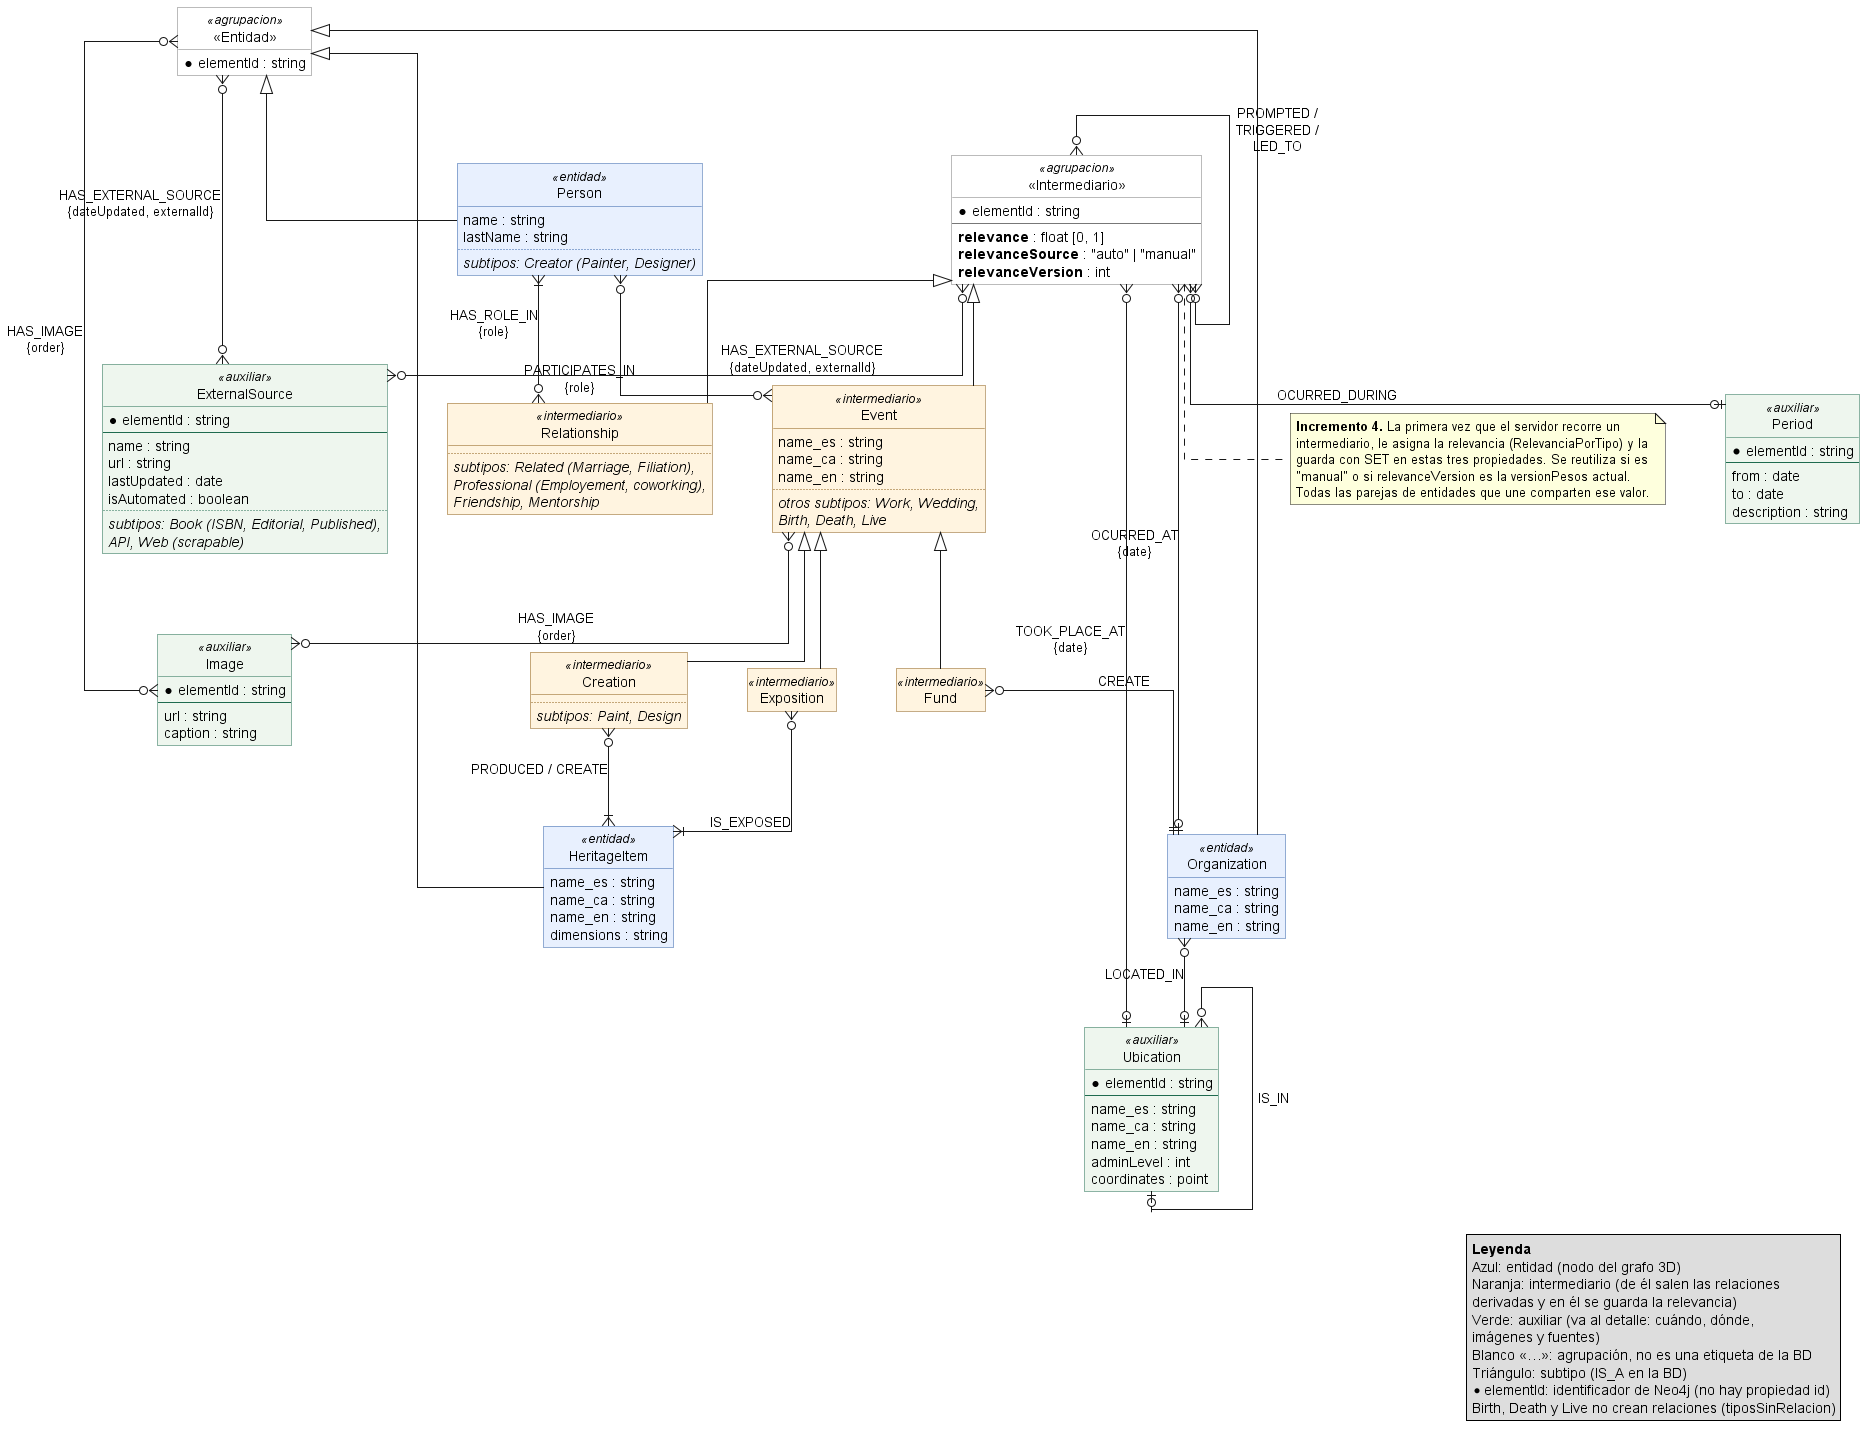
\includegraphics[width=\textwidth]{diagramas/bd_refracts.png}
  \caption{Modelo de datos de REFRACTS en Neo4j, con las propiedades de relevancia que añade la aplicación.}
  \label{fig:bd-refracts}
\end{figure}

\begin{table}[htbp]
  \centering
  \caption{Etiquetas de REFRACTS y papel que les da la aplicación.}
  \label{tab:etiquetas}
  \begin{tabular}{@{}llp{6.2cm}@{}}
    \toprule
    Etiqueta & Papel & Propiedades \\
    \midrule
    \texttt{Person} & entidad & \texttt{name}, \texttt{lastName} \\
    \texttt{Organization} & entidad & \texttt{name\_es}, \texttt{name\_ca}, \texttt{name\_en} \\
    \texttt{HeritageItem} & entidad & \texttt{name\_es/ca/en}, \texttt{dimensions} \\
    \texttt{Relationship} y subtipos & intermediario & \texttt{relevance}, \texttt{relevanceSource}, \texttt{relevanceVersion} (añadidas) \\
    \texttt{Event} y subtipos & intermediario & \texttt{name\_es/ca/en} y las tres de relevancia \\
    \texttt{Period} & auxiliar & \texttt{from}, \texttt{to}, \texttt{description} \\
    \texttt{Ubication} & auxiliar & \texttt{name\_es/ca/en}, \texttt{adminLevel}, \texttt{coordinates} \\
    \texttt{Image} & auxiliar & \texttt{url}, \texttt{caption} \\
    \texttt{ExternalSource} & auxiliar & \texttt{name}, \texttt{url}, \texttt{lastUpdated}, \texttt{isAutomated} \\
    \bottomrule
  \end{tabular}
\end{table}

\subsection{Modelo derivado que usa la aplicación}

El visor no trabaja con el grafo de REFRACTS, sino con un grafo de entidades unidas directamente por relaciones derivadas (sección~\ref{sec:alg-derivadas}). La figura~\ref{fig:bd-derivacion} muestra la transformación con un ejemplo: dos personas unidas por un intermediario \texttt{Marriage} pasan a estar unidas por una relación de tipo \texttt{Marriage} con los roles de cada una y el periodo del intermediario; una persona y una obra unidas por una \texttt{Creation} (en este caso, \texttt{Paint}) pasan a estar unidas por una relación de tipo \texttt{Paint}. El valor de cada relación derivada es la relevancia guardada en su intermediario, de modo que todas las parejas que salen del mismo intermediario comparten valor.

\begin{figure}[htbp]
  \centering
  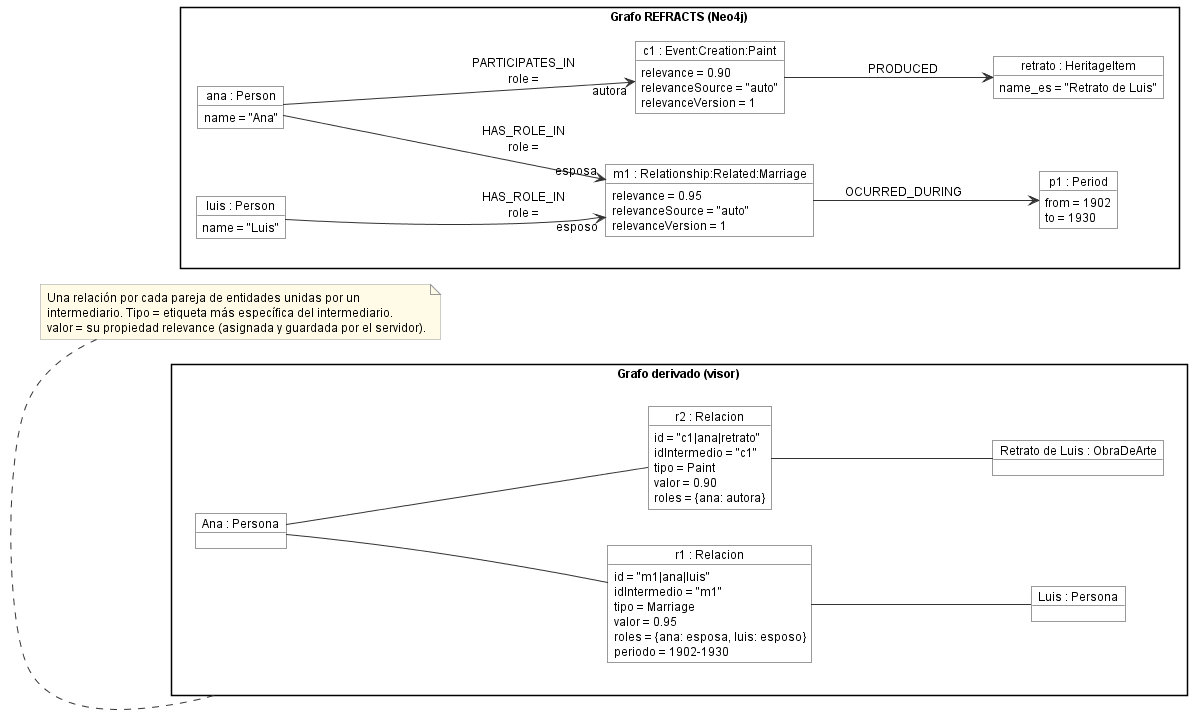
\includegraphics[width=\textwidth]{diagramas/bd_derivacion.png}
  \caption{Del grafo de REFRACTS (arriba) al grafo derivado que recibe el visor (abajo).}
  \label{fig:bd-derivacion}
\end{figure}

La figura~\ref{fig:bd-app} resume, como diagrama entidad--relación, el modelo de datos con el que trabaja el cliente: los datos del grafo (entidades, relaciones derivadas y sus tipos), lo que calcula el visor (subgrafo y nodos con su relevancia, nivel y centralidad) y el detalle que se pide al seleccionar una entidad (eventos, imágenes y fuentes).

\begin{figure}[htbp]
  \centering
  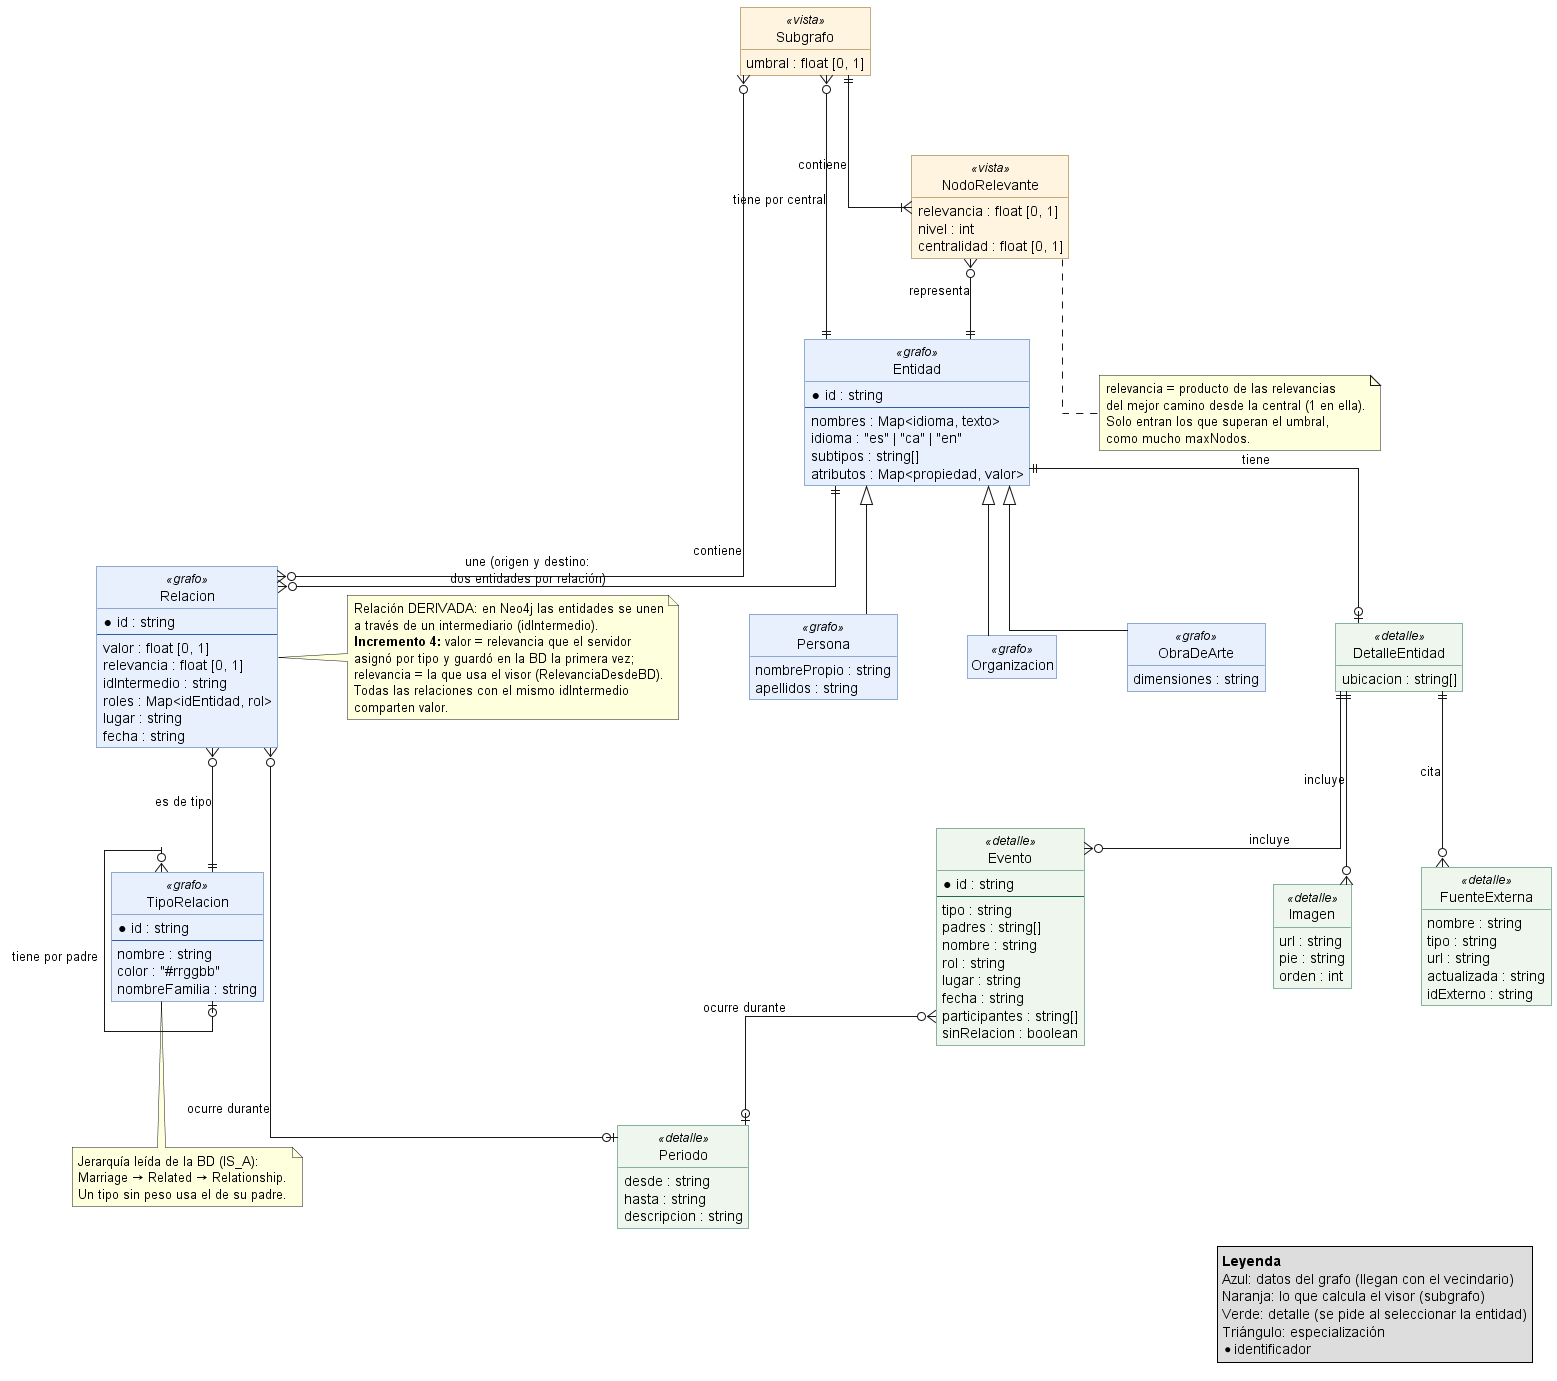
\includegraphics[width=\textwidth]{diagramas/bd_modelo_app.png}
  \caption{Modelo de datos de la aplicación (cliente).}
  \label{fig:bd-app}
\end{figure}

\subsection{Propiedades que añade la aplicación}

La aplicación añade tres propiedades: \texttt{relevance} (real en $[0,1]$), \texttt{relevanceSource} (\texttt{auto} o \texttt{manual}) y \texttt{relevanceVersion} (entero). Se guardan en el elemento de la base de datos que produce la relación: en el nodo intermediario, para las relaciones por intermediario, y en la propia relación de Neo4j, para las relaciones directas entre entidades, que el diseño actual de REFRACTS no tiene pero la regla admite (los datos simulados incluyen una, \texttt{STUDENT\_OF}, para probarlo).

Guardarlas en el intermediario, y no en cada pareja derivada, tiene dos ventajas. Las parejas derivadas no existen en la base de datos; guardarlas obligaría a materializar $p(p-1)/2$ relaciones por intermediario y a mantenerlas cuando cambian los participantes. Además, la relevancia depende del tipo del vínculo, que es una propiedad del intermediario, así que todas sus parejas deben tener el mismo valor.

\subsection{Consultas}

Las consultas a Neo4j se implementan en el incremento~4 en \texttt{RepositorioNeo4j} y \texttt{AlmacenRelevanciasNeo4j}, que sustituyen a \texttt{RepositorioSimulado} y \texttt{AlmacenRelevanciasEnGrafo} sin cambiar las demás clases. Las listas de etiquetas y tipos se pasan como parámetros desde la configuración, nunca escritas en la consulta. El listado~\ref{lst:cypher-vecindario} obtiene, para toda la frontera de un nivel del recorrido, los intermediarios y sus participantes.

\begin{lstlisting}[style=codigo, caption={Consulta prevista: intermediarios de la frontera de un nivel.}, label={lst:cypher-vecindario}]
UNWIND $frontera AS idEntidad
MATCH (e) WHERE elementId(e) = idEntidad
MATCH (e)-[r1]-(i)
WHERE NOT type(r1) IN $relacionesIgnoradas
  AND NONE(l IN labels(i) WHERE l IN $etiquetasEntidad
                             OR l IN $etiquetasAuxiliares
                             OR l IN $tiposSinRelacion)
MATCH (i)-[r2]-(otra)
WHERE NOT type(r2) IN $relacionesIgnoradas
  AND ANY(l IN labels(otra) WHERE l IN $etiquetasEntidad)
WITH idEntidad, i, collect(DISTINCT {id: elementId(otra), rol: r2.role}) AS participantes
WHERE size(participantes) <= $maxParticipantes
RETURN idEntidad, elementId(i) AS idIntermedio, labels(i) AS etiquetas,
       i.relevance AS relevance, i.relevanceSource AS fuente,
       i.relevanceVersion AS version, participantes
\end{lstlisting}
% TODO: comprobar la consulta con la BD real; añadir las relaciones directas, el periodo, el lugar y la fecha del intermediario.

El listado~\ref{lst:cypher-guardar} guarda una relevancia calculada. La escritura es condicional: solo se hace si el valor no es manual y no está ya calculado con la versión actual de los pesos. \texttt{coalesce} trata como «automático, versión 0» un intermediario que todavía no tiene las propiedades. Si dos peticiones simultáneas calculan la relevancia del mismo intermediario, Neo4j serializa las dos escrituras sobre el nodo; la segunda ya no cumple la condición y no escribe, y como ambas calculan el mismo valor, el resultado no depende del orden.

\begin{lstlisting}[style=codigo, caption={Consulta prevista: guardar la relevancia sin pisar un valor manual.}, label={lst:cypher-guardar}]
MATCH (i) WHERE elementId(i) = $id
  AND coalesce(i.relevanceSource, 'auto') <> 'manual'
  AND coalesce(i.relevanceVersion, 0) < $version
SET i.relevance = $valor,
    i.relevanceSource = 'auto',
    i.relevanceVersion = $version
\end{lstlisting}
% TODO: comprobar el comportamiento concurrente con la edición de Neo4j que use el IRTIC.

\subsection{Configuración}

La clasificación de las etiquetas, los límites de la regla y la tabla de pesos están en \texttt{servidor/configuracion.json} (listado~\ref{lst:configuracion}), que el servidor valida al arrancar (\texttt{Configuracion.comprobar}). Añadir un tipo de evento o de relación a REFRACTS no exige cambiar el código: el tipo nuevo se trata como intermediario y recibe el peso de su padre más cercano. Si se quiere un peso propio, basta con añadirlo a \texttt{pesosRelevancia} y subir \texttt{versionPesos}, con lo que las relevancias automáticas antiguas se recalculan la próxima vez que se recorran. Esto cumple RNF-16 y mejora la mantenibilidad: los cambios en el modelo de datos se resuelven en la configuración, no en el código.

\begin{lstlisting}[style=codigo, caption={Fragmento de \texttt{configuracion.json}.}, label={lst:configuracion}]
"etiquetasEntidad":    { "Person": "PERSONA", "Organization": "ORGANIZACION",
                         "HeritageItem": "OBRA_DE_ARTE" },
"etiquetasAuxiliares": ["Period", "Ubication", "Image", "ExternalSource"],
"tiposSinRelacion":    ["Birth", "Death", "Live"],
"relacionesIgnoradas": ["IS_A", "IS_IN", "LOCATED_IN", "HAS_IMAGE",
                        "HAS_EXTERNAL_SOURCE", "PROMPTED", "TRIGGERED", "LED_TO"],
"maxParticipantesIntermediario": 10,
"pesosRelevancia": { "Marriage": 0.95, "Filiation": 0.90, "Mentorship": 0.85, ... },
"pesoPorDefecto": 0.5,
"versionPesos": 1
\end{lstlisting}

\subsection{Seguridad y permisos}

RNF-11 establece que la aplicación accede a la base de datos solo en lectura, pero la asignación perezosa necesita escribir las tres propiedades de relevancia. Hay dos opciones, que se deben decidir con el IRTIC:
\begin{enumerate}
  \item Conceder al usuario de la aplicación permiso de escritura solo sobre las propiedades \texttt{relevance}, \texttt{relevanceSource} y \texttt{relevanceVersion}. El control de acceso por propiedad está disponible en Neo4j Enterprise, no en la edición Community. \cite{TODO}
  \item Mantener Neo4j en solo lectura y guardar las relevancias en un almacén propio de la aplicación (por ejemplo, SQLite). El diseño ya lo permite: \texttt{AsignadorRelevancia} solo conoce la interfaz \texttt{AlmacenRelevancias}, y bastaría con otra implementación.
\end{enumerate}
% TODO: decidir la opción con el IRTIC y actualizar RNF-11.

Las credenciales de Neo4j se leen de variables de entorno (fichero \texttt{.env}, excluido del control de versiones) y no aparecen en \texttt{configuracion.json}. Las consultas usan parámetros, nunca concatenación de texto, lo que evita la inyección de Cypher. El tratamiento de datos de personas vivas (RNF-23) queda pendiente de definir con el IRTIC. % TODO: RNF-23.

\subsection{Datos simulados}

Para desarrollar y probar sin acceso a Neo4j, \texttt{RepositorioSimulado} implementa la misma interfaz \texttt{RepositorioDatos} sobre un fichero JSON con la misma forma que el grafo de REFRACTS: nodos con etiquetas y propiedades, relaciones con tipo y propiedades, y la jerarquía \texttt{IS\_A}. Las relevancias se guardan en memoria en las propiedades de los nodos (\texttt{AlmacenRelevanciasEnGrafo}), igual que se harán en Neo4j. El fichero lo genera \texttt{generar\_datos\_ejemplo.py} con semilla fija (2026), de modo que las pruebas son reproducibles. Contiene 1462 nodos (120 \texttt{Person}, 25 \texttt{Organization}, 60 \texttt{HeritageItem}, 190 \texttt{Relationship}, 389 \texttt{Event}, 514 \texttt{Period}, 143 \texttt{Image}, 15 \texttt{Ubication} y 6 \texttt{ExternalSource}) y 2500 relaciones. Incluye a propósito casos que no están en el diseño de REFRACTS pero que la regla debe tratar: dos congresos con 14 asistentes (por encima del límite de participantes), un tipo sin peso propio (\texttt{Apprenticeship}, que hereda el de \texttt{Professional}) y relaciones directas entre personas (\texttt{STUDENT\_OF}).

\subsection{Dudas abiertas sobre la base de datos}
\label{sec:bd-dudas}

\begin{itemize}
  \item Erratas en los nombres: \texttt{Ubication}, \texttt{Employement}, \texttt{OCURRED\_AT} y \texttt{OCURRED\_DURING}, \texttt{coworking} en minúsculas y espacios al final de algunas etiquetas. La aplicación usa los nombres tal como estén; si se corrigen, solo hay que actualizar la configuración.
  \item \texttt{Creation} se une a \texttt{HeritageItem} con dos relaciones, \texttt{PRODUCED} y \texttt{CREATE}. ¿Son equivalentes?
  \item ¿Los subtipos son varias etiquetas en el mismo nodo (\texttt{:Event:Creation:Paint}) o nodos de una taxonomía? Cambia cómo se lee la jerarquía.
  \item No hay un identificador propio; se usa \texttt{elementId}, que Neo4j no garantiza estable entre versiones. Un identificador estable es necesario para enlazar entidades desde fuera.
  \item Tamaño de la base de datos: \texttt{/api/nombres} descarga el índice de nombres completo al arrancar, lo que puede no ser viable si hay cientos de miles de entidades.
  \item Permisos de escritura y edición de Neo4j (sección anterior).
\end{itemize}

% ----------------------------------------------------------------------------
\section{Diagrama de clases de diseño}
\label{sec:clases}

Los diagramas se han obtenido del código actual. Para representar en UML las clases de JavaScript se usan las equivalencias de la tabla~\ref{tab:equivalencias}. En Python, los miembros con doble guion bajo (\texttt{\_\_x}) se representan como privados y las clases que heredan de \texttt{ABC} con métodos \texttt{@abstractmethod}, como abstractas.

\begin{table}[htbp]
  \centering
  \caption{Equivalencias entre JavaScript y UML.}
  \label{tab:equivalencias}
  \begin{tabular}{@{}ll@{}}
    \toprule
    JavaScript & UML \\
    \midrule
    campo o método \texttt{\#x} & privado (\texttt{-}) \\
    campo o método \texttt{\_x} & protegido (\texttt{\#}) \\
    resto & público (\texttt{+}) \\
    \texttt{static} & miembro de clase (subrayado) \\
    clase que impide \texttt{new} con \texttt{new.target} & \texttt{\{abstract\}} \\
    clase base cuyos métodos lanzan «No implementado» & \texttt{<<interface>>} \\
    objeto congelado con \texttt{Object.freeze} & \texttt{<<enumeration>>} \\
    \bottomrule
  \end{tabular}
\end{table}

\subsection{Servidor}

La figura~\ref{fig:clases-servidor} muestra las clases del servidor. El módulo \texttt{app} define las rutas de FastAPI y crea las dependencias al arrancar. El paquete \texttt{api} contiene la caché (\texttt{CacheRespuestas}) y la conversión a JSON (\texttt{ConversorJson}). El paquete \texttt{logica} contiene la configuración, la clasificación de etiquetas y el cálculo de relevancias (\texttt{EstrategiaRelevancia}, \texttt{RelevanciaPorTipo} y \texttt{AsignadorRelevancia}). El paquete \texttt{datos} contiene los repositorios, la regla de relaciones derivadas (\texttt{ProyectorRelaciones}) y los almacenes de relevancia. Las clases marcadas como «previsto incremento~4» son las que conectan con Neo4j.

\begin{figure}[htbp]
  \centering
  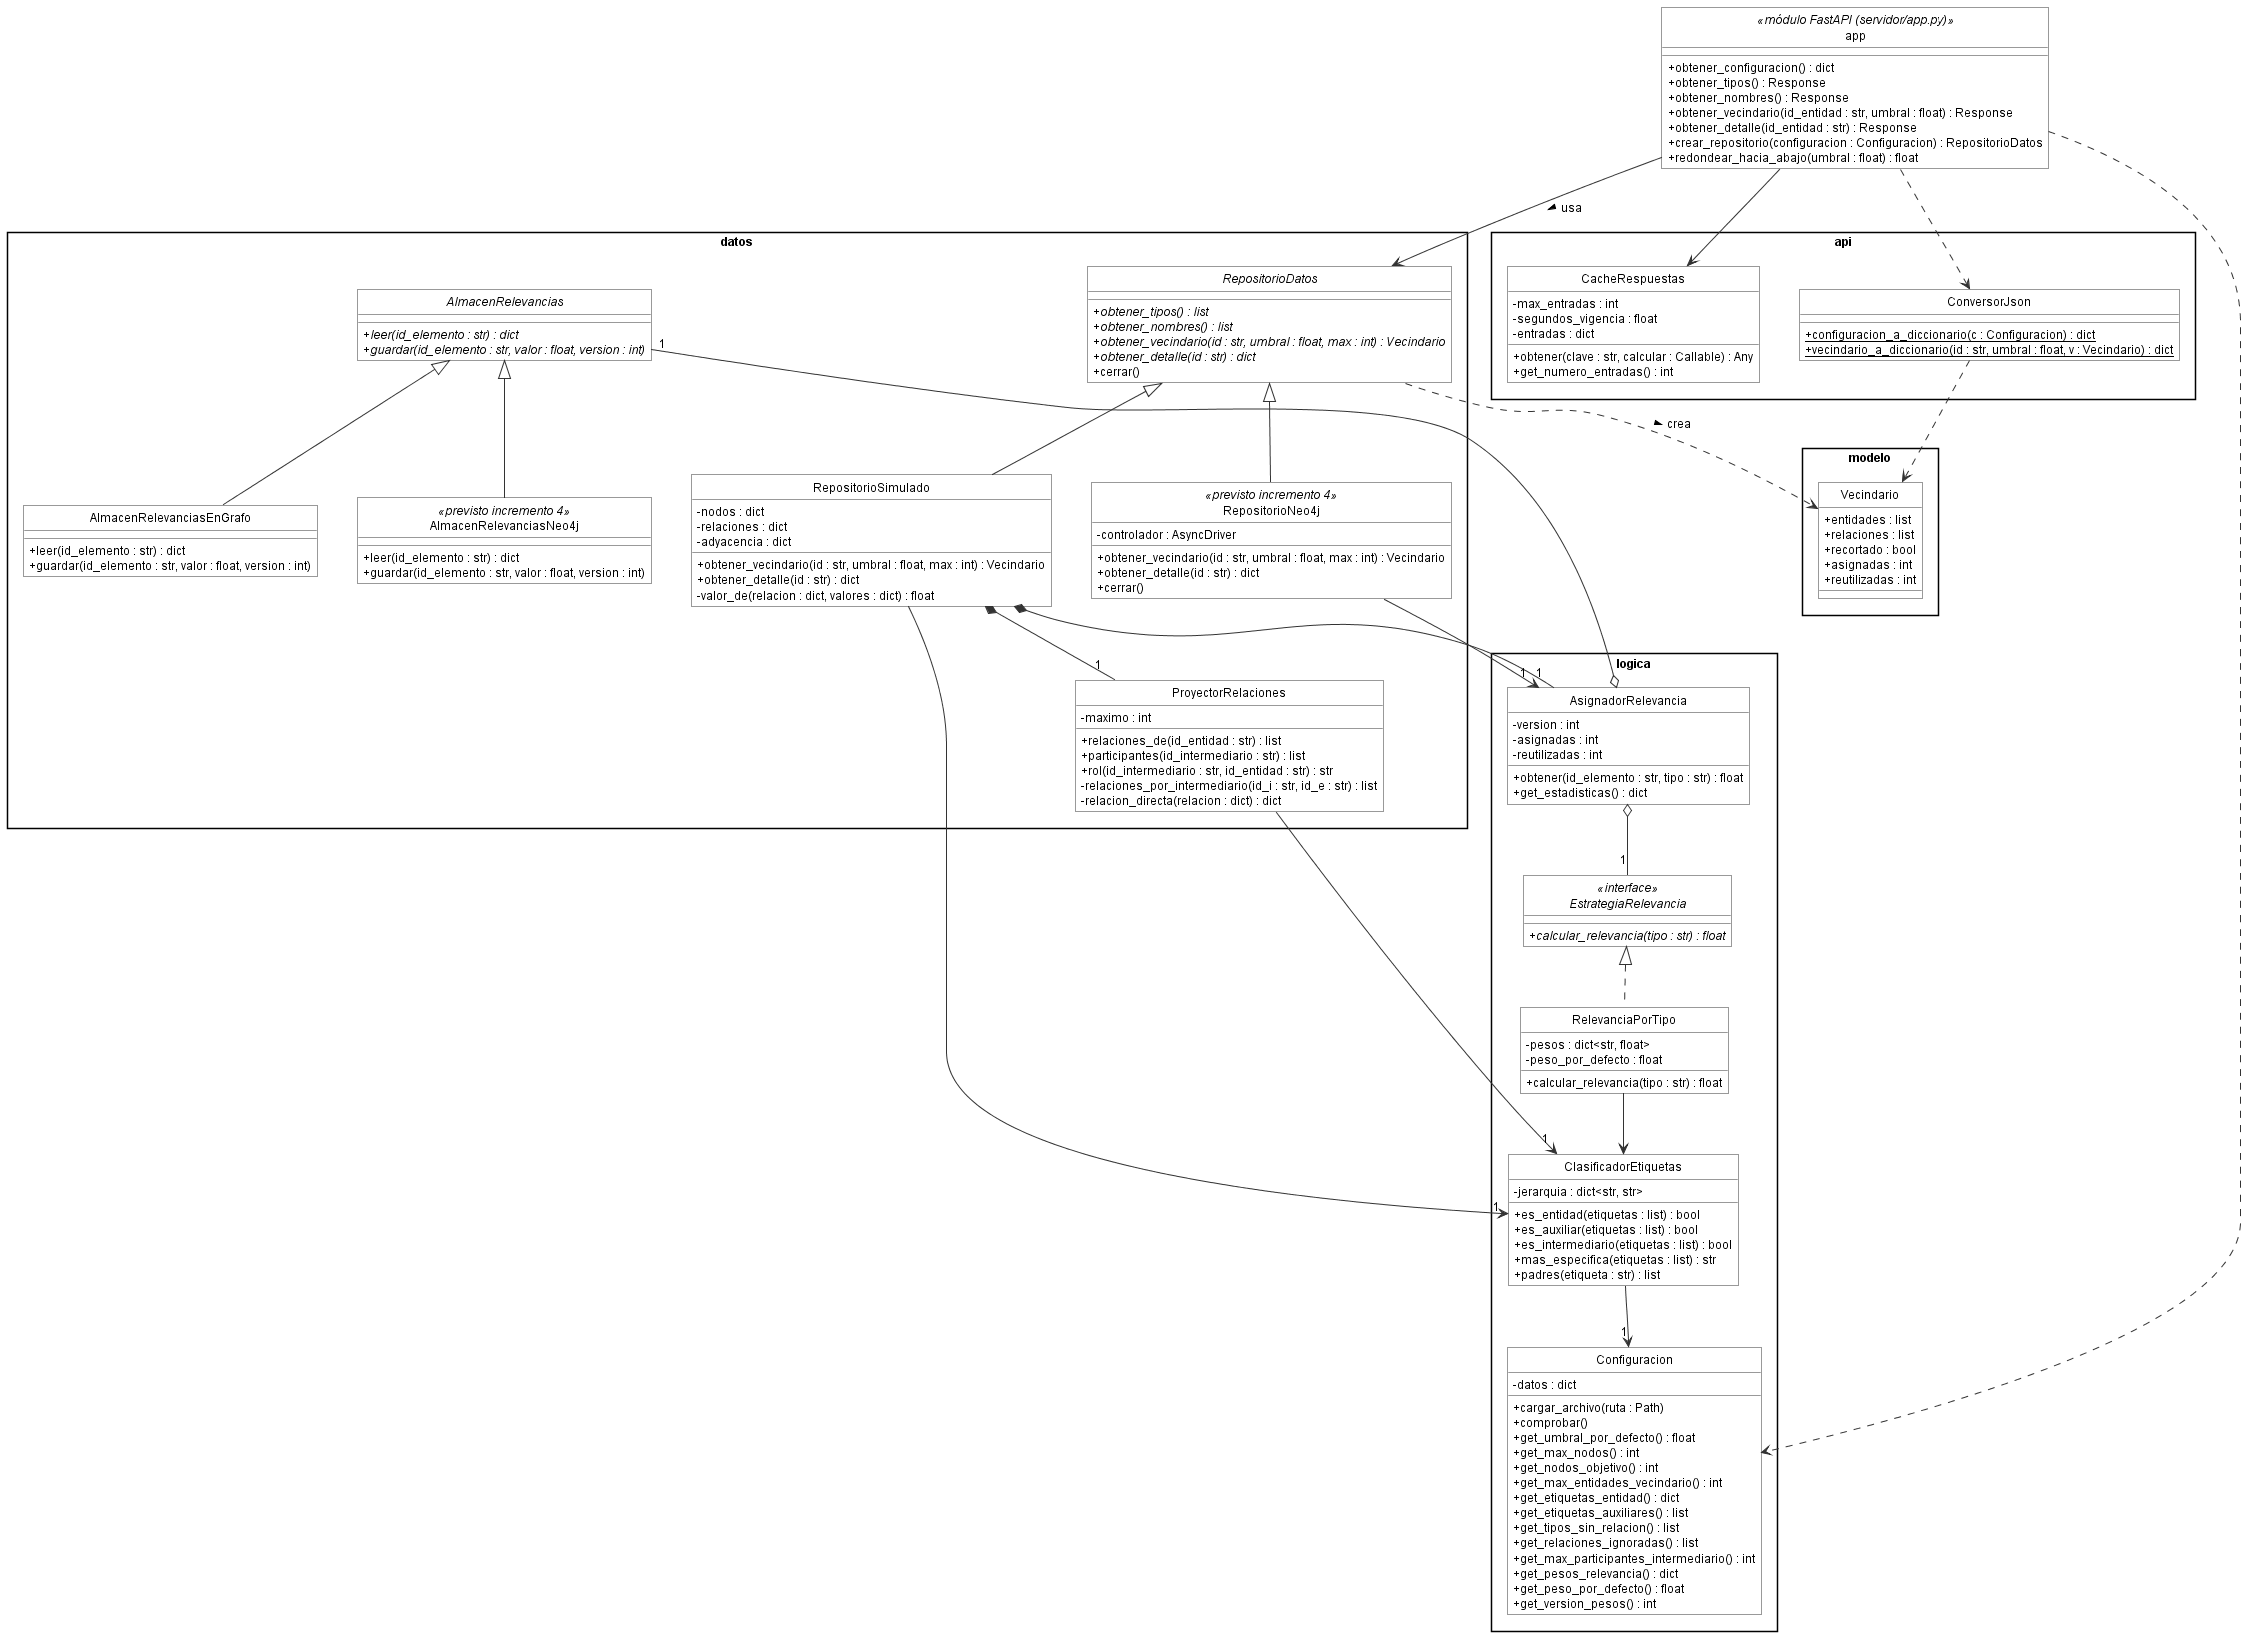
\includegraphics[width=\textwidth]{diagramas/clases_servidor.png}
  \caption{Diagrama de clases del servidor.}
  \label{fig:clases-servidor}
\end{figure}

El paquete \texttt{servidor/modelo} conserva clases del incremento~2 (\texttt{Entidad}, \texttt{Persona}, \texttt{Subgrafo}, \texttt{NodoRelevante}\ldots) y \texttt{datos/fabrica\_entidades.py}, de cuando el servidor construía el subgrafo. Desde el incremento~3 solo se usa \texttt{Vecindario}; las demás solo las usan las pruebas y no aparecen en el diagrama. % TODO: decidir si se eliminan del código.

\subsection{Cliente}

La figura~\ref{fig:clases-cliente} muestra las clases del cliente y sus relaciones, sin miembros. Las figuras siguientes detallan cada paquete.

\begin{figure}[htbp]
  \centering
  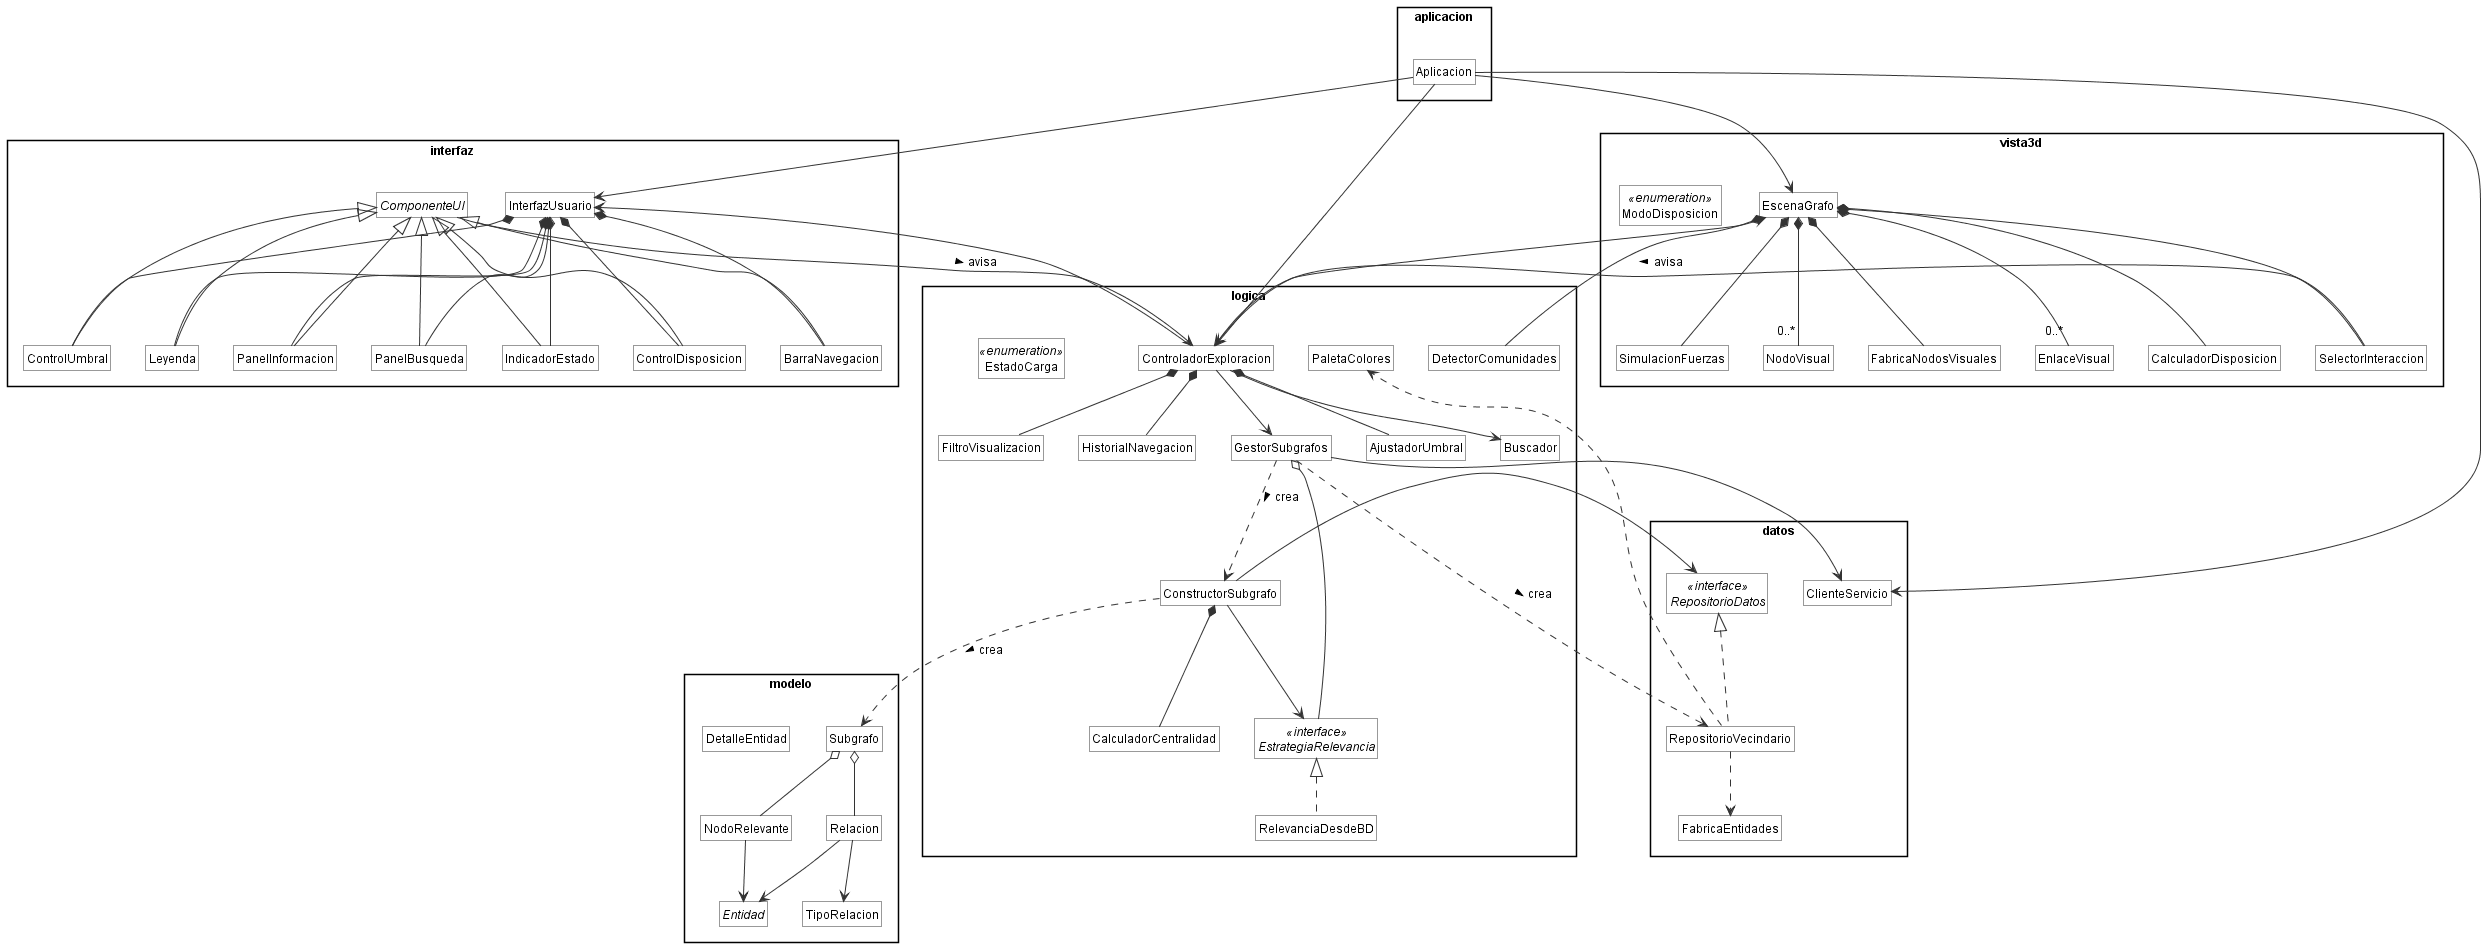
\includegraphics[width=\textwidth]{diagramas/clases_cliente_general.png}
  \caption{Diagrama de clases general del cliente.}
  \label{fig:clases-cliente}
\end{figure}

\paragraph{modelo} (figura~\ref{fig:clases-modelo}). Las clases del dominio, sin dependencias de otros paquetes. \texttt{Entidad} es abstracta, con las subclases \texttt{Persona}, \texttt{Organizacion} y \texttt{ObraDeArte}; guarda los nombres en varios idiomas, los subtipos (etiquetas de Neo4j distintas de la principal) y los atributos que la clase no conoce, para que una propiedad nueva de la base de datos se muestre sin cambiar el código. \texttt{Relacion} es la relación derivada, con su valor, su relevancia, el intermediario y los roles. \texttt{Subgrafo} agrega los \texttt{NodoRelevante} y las relaciones seleccionadas. \texttt{DetalleEntidad} agrupa lo que se pide al seleccionar una entidad.

\begin{figure}[htbp]
  \centering
  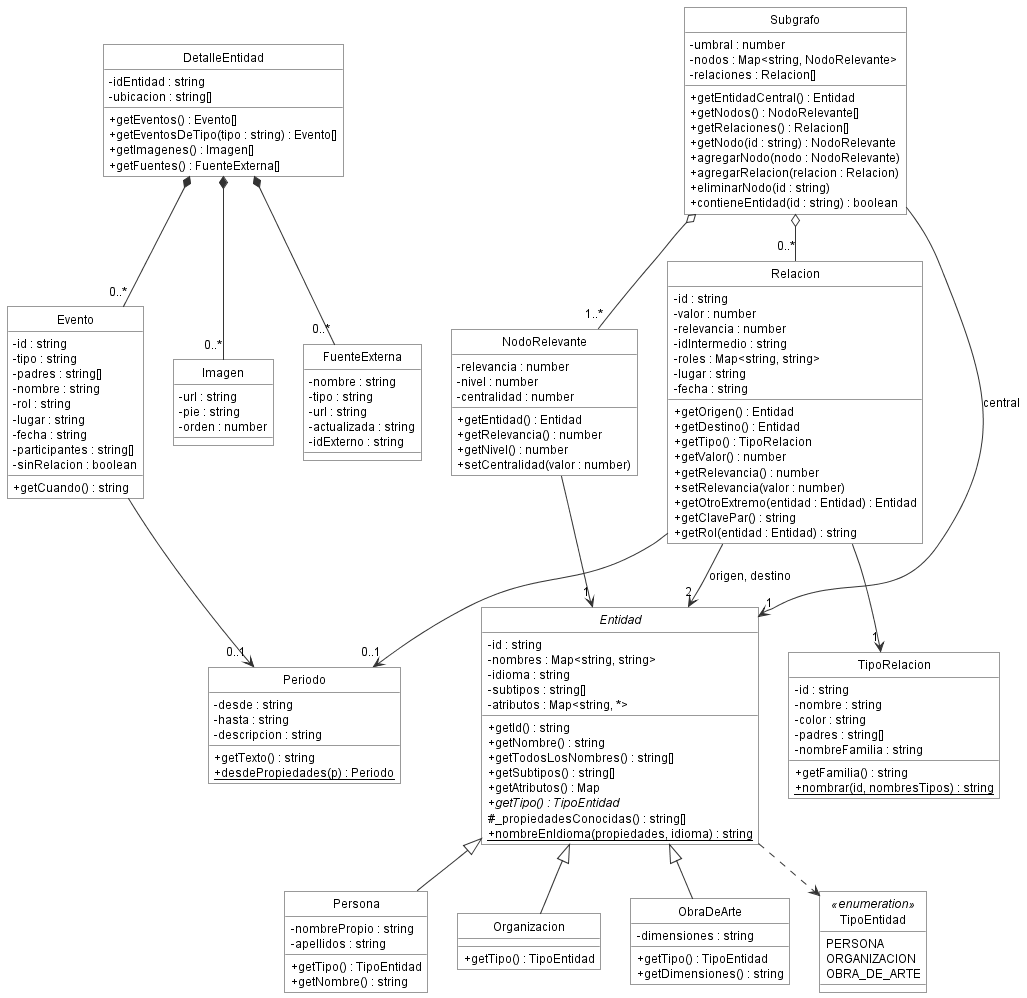
\includegraphics[width=\textwidth]{diagramas/clases_modelo.png}
  \caption{Paquete \texttt{modelo}.}
  \label{fig:clases-modelo}
\end{figure}

\paragraph{datos} (figura~\ref{fig:clases-datos}). \texttt{ClienteServicio} es la única clase que hace peticiones HTTP. \texttt{RepositorioDatos} es la interfaz con la que \texttt{ConstructorSubgrafo} lee entidades y relaciones; \texttt{RepositorioVecindario} la implementa en memoria sobre un vecindario recibido, con un índice de relaciones por entidad que hace que cada expansión cueste $O(\text{grado})$. \texttt{FabricaEntidades} crea la subclase de \texttt{Entidad} que corresponde a las etiquetas.

\begin{figure}[htbp]
  \centering
  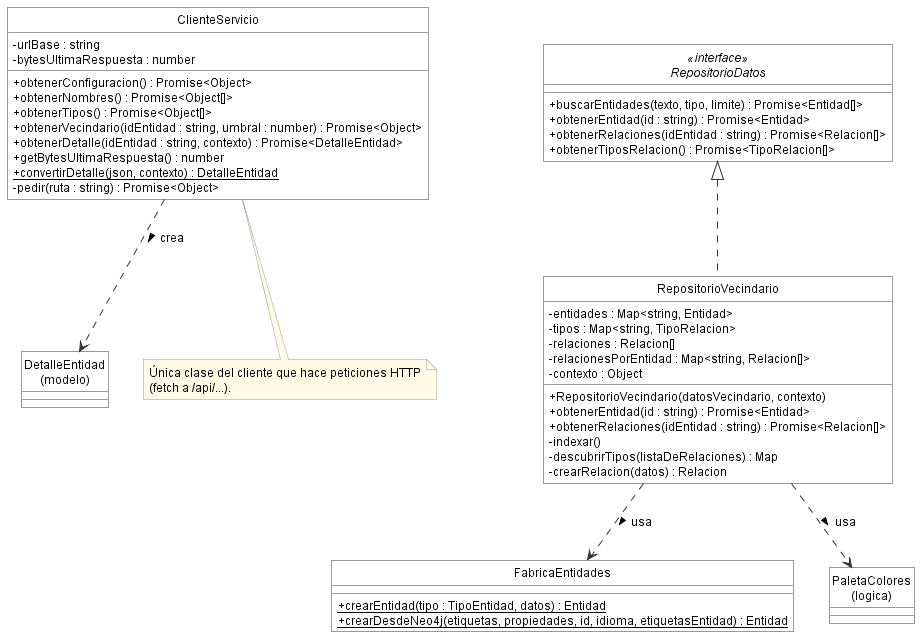
\includegraphics[width=0.85\textwidth]{diagramas/clases_datos.png}
  \caption{Paquete \texttt{datos}.}
  \label{fig:clases-datos}
\end{figure}

\paragraph{logica} (figuras~\ref{fig:clases-logica-subgrafo} y~\ref{fig:clases-logica-control}). Se divide en dos diagramas. El primero contiene el cálculo: \texttt{GestorSubgrafos} (obtención y reutilización del vecindario), \texttt{ConstructorSubgrafo}, la estrategia de relevancia, \texttt{CalculadorCentralidad}, \texttt{AjustadorUmbral}, \texttt{Buscador}, \texttt{PaletaColores} y \texttt{DetectorComunidades}. El segundo, el control: \texttt{ControladorExploracion} con \texttt{FiltroVisualizacion} y \texttt{HistorialNavegacion}, que nacen y mueren con él.

\begin{figure}[htbp]
  \centering
  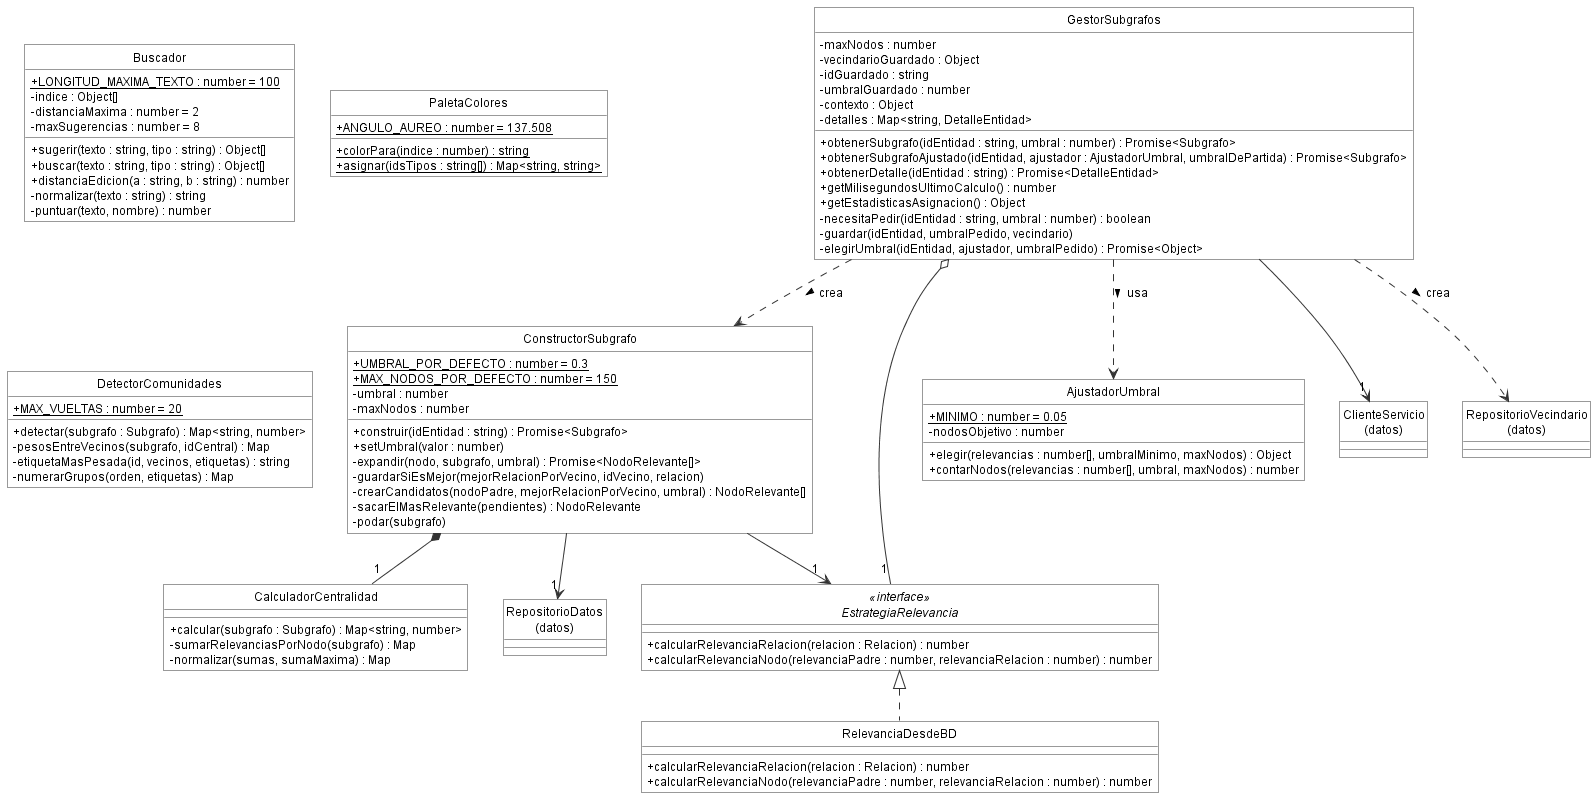
\includegraphics[width=\textwidth]{diagramas/clases_logica_subgrafo.png}
  \caption{Paquete \texttt{logica}: obtención y cálculo del subgrafo.}
  \label{fig:clases-logica-subgrafo}
\end{figure}

\begin{figure}[htbp]
  \centering
  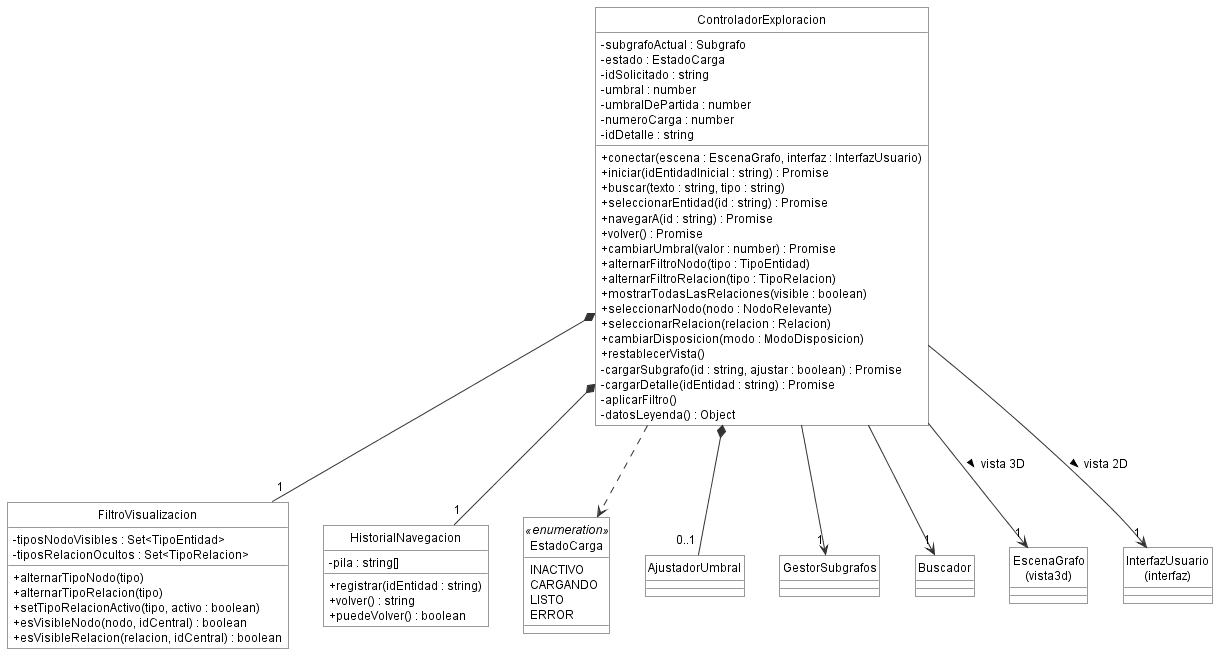
\includegraphics[width=0.85\textwidth]{diagramas/clases_logica_control.png}
  \caption{Paquete \texttt{logica}: control de la exploración.}
  \label{fig:clases-logica-control}
\end{figure}

\paragraph{vista3d} (figura~\ref{fig:clases-vista3d}). \texttt{EscenaGrafo} es la vista 3D: crea la escena de Three.js, los nodos y enlaces visuales, la simulación y el selector de interacción, y los anima en cada fotograma. \texttt{NodoVisual} es abstracta; sus subclases solo definen la geometría y el color de cada tipo de entidad (esfera, cubo, octaedro). \texttt{SelectorInteraccion} traduce los eventos del puntero en llamadas al controlador.

\begin{figure}[htbp]
  \centering
  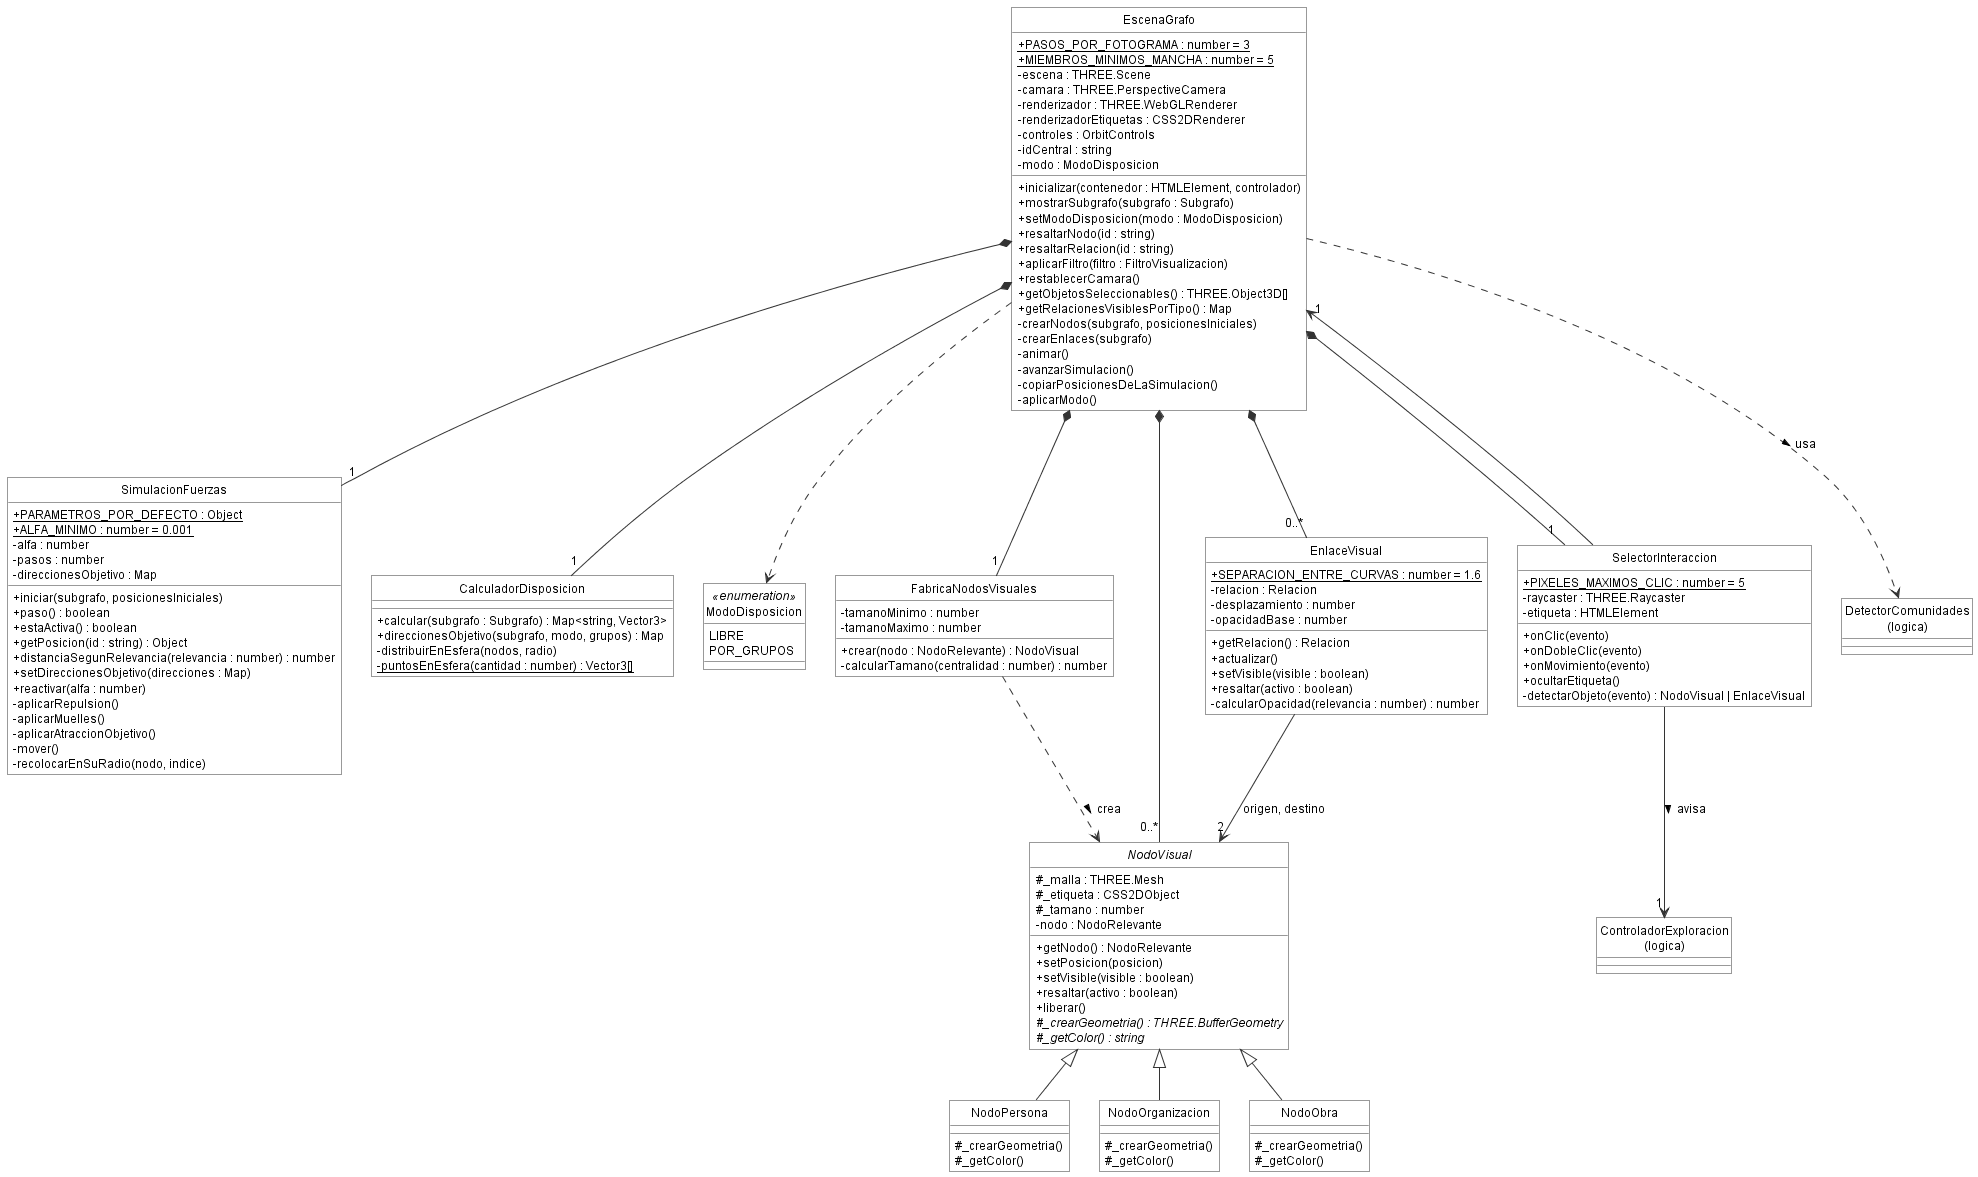
\includegraphics[width=\textwidth]{diagramas/clases_vista3d.png}
  \caption{Paquete \texttt{vista3d}.}
  \label{fig:clases-vista3d}
\end{figure}

\paragraph{interfaz y aplicacion} (figura~\ref{fig:clases-interfaz}). \texttt{InterfazUsuario} compone los siete paneles de la interfaz 2D, todos subclases de \texttt{ComponenteUI}. \texttt{Aplicacion} es el punto de entrada: pide la configuración, los nombres y los tipos, y crea y conecta todas las piezas.

\begin{figure}[htbp]
  \centering
  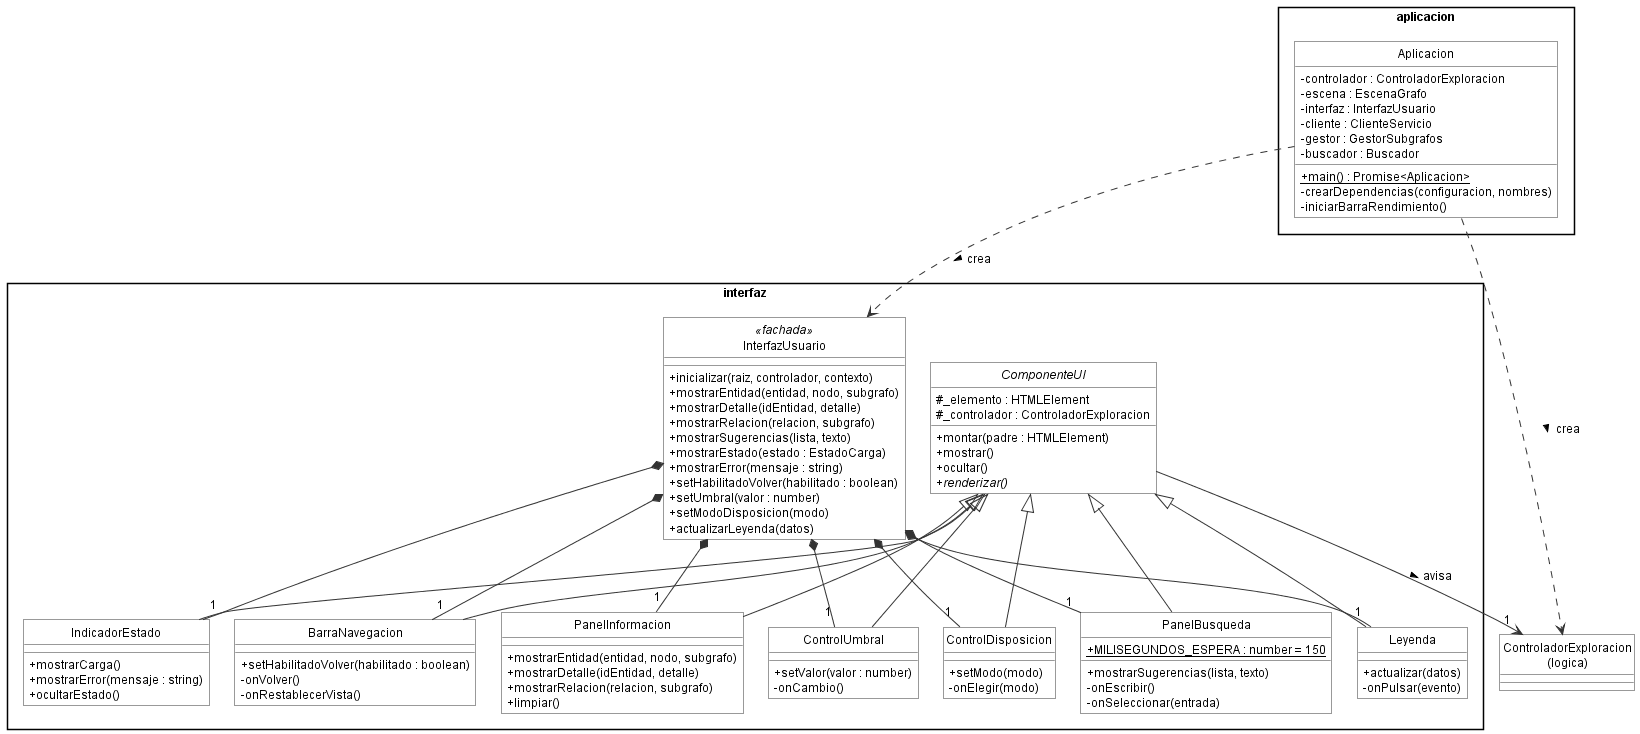
\includegraphics[width=\textwidth]{diagramas/clases_interfaz.png}
  \caption{Paquetes \texttt{interfaz} y \texttt{aplicacion}.}
  \label{fig:clases-interfaz}
\end{figure}

\subsection{Patrones y principios de diseño}
\label{sec:patrones}

\paragraph{Estrategia.} La forma de medir la relevancia es la decisión más discutible del sistema y la que más probablemente cambie. Por eso se aísla detrás de una interfaz en los dos lados: en el servidor, \texttt{EstrategiaRelevancia} con \texttt{RelevanciaPorTipo}; en el cliente, \texttt{EstrategiaRelevancia} con \texttt{RelevanciaDesdeBD}. Una medida nueva se añade como otra implementación sin modificar \texttt{AsignadorRelevancia} ni \texttt{ConstructorSubgrafo} (principio abierto/cerrado).

\paragraph{Fábrica.} \texttt{FabricaEntidades} crea la subclase de \texttt{Entidad} a partir de las etiquetas, y \texttt{FabricaNodosVisuales} crea el \texttt{NodoVisual} adecuado a cada tipo y calcula su tamaño. Así la decisión «qué clase corresponde a este tipo» está en un solo sitio, y el resto del código trabaja con la clase base sin preguntar por el tipo.

\paragraph{Método plantilla.} \texttt{NodoVisual} implementa el comportamiento común (posición, visibilidad, resaltado, etiqueta) y delega en las subclases solo \texttt{\_crearGeometria} y \texttt{\_getColor}.

\paragraph{Modelo--vista--controlador.} \texttt{ControladorExploracion} recibe todo lo que hace el usuario, tanto desde la escena (\texttt{SelectorInteraccion}) como desde los paneles (\texttt{ComponenteUI}), decide qué hacer y se lo pide al modelo (\texttt{GestorSubgrafos}, \texttt{Buscador}, \texttt{FiltroVisualizacion}, \texttt{HistorialNavegacion}) o a las vistas (\texttt{EscenaGrafo}, \texttt{InterfazUsuario}). Las vistas no se comunican entre sí ni con el modelo, lo que reduce el acoplamiento: por ejemplo, la vista 3D no sabe que existe un panel de información.

\paragraph{Fachada.} \texttt{InterfazUsuario} ofrece al controlador una sola interfaz (\texttt{mostrarEntidad}, \texttt{mostrarEstado}, \texttt{setUmbral}\ldots) y reparte cada llamada al panel que corresponde. El controlador no conoce los siete paneles; si se cambia la distribución de la interfaz, el controlador no se modifica.

\paragraph{Repositorio e inversión de dependencias.} Las clases que necesitan datos dependen de interfaces, no de implementaciones concretas: \texttt{ConstructorSubgrafo} de \texttt{RepositorioDatos} (cliente), \texttt{app} de \texttt{RepositorioDatos} (servidor) y \texttt{AsignadorRelevancia} de \texttt{AlmacenRelevancias}. Es lo que permite pasar de los datos simulados a Neo4j en el incremento~4 sustituyendo dos clases, y lo que permitiría la segunda opción de permisos (almacén propio) sin tocar el resto (RNF-17).

\paragraph{Inyección de dependencias.} En el cliente, \texttt{Aplicacion.\#crearDependencias} es el único sitio donde se crean las clases principales, que reciben sus colaboradores en el constructor. Las pruebas aprovechan esto para sustituir, por ejemplo, \texttt{ClienteServicio} por un doble que no accede a la red.

% ----------------------------------------------------------------------------
\section{Diagramas de interacción}
\label{sec:interaccion}

Cada operación del sistema se describe con un diagrama de secuencia cuyos participantes y mensajes son las clases y métodos de la sección~\ref{sec:clases}. Las llamadas HTTP entre el navegador y el servidor aparecen como mensajes \texttt{GET}. Los métodos privados se escriben con \texttt{\#}, como en el código. Las operaciones son las de los casos de uso del capítulo~3. % TODO: poner los identificadores CU-xx de cada operación.

\subsection{Cargar la aplicación}

Al abrir la página (figura~\ref{fig:sec-cargar}), \texttt{Aplicacion.main} pide en paralelo la configuración, el índice de nombres y la jerarquía de tipos, con \texttt{Promise.all}. Pedirlas en paralelo reduce el tiempo de arranque al de la petición más lenta, en vez de la suma de las tres. Después crea las dependencias, conecta el controlador con las dos vistas y carga la entidad inicial de la configuración.

\begin{figure}[htbp]
  \centering
  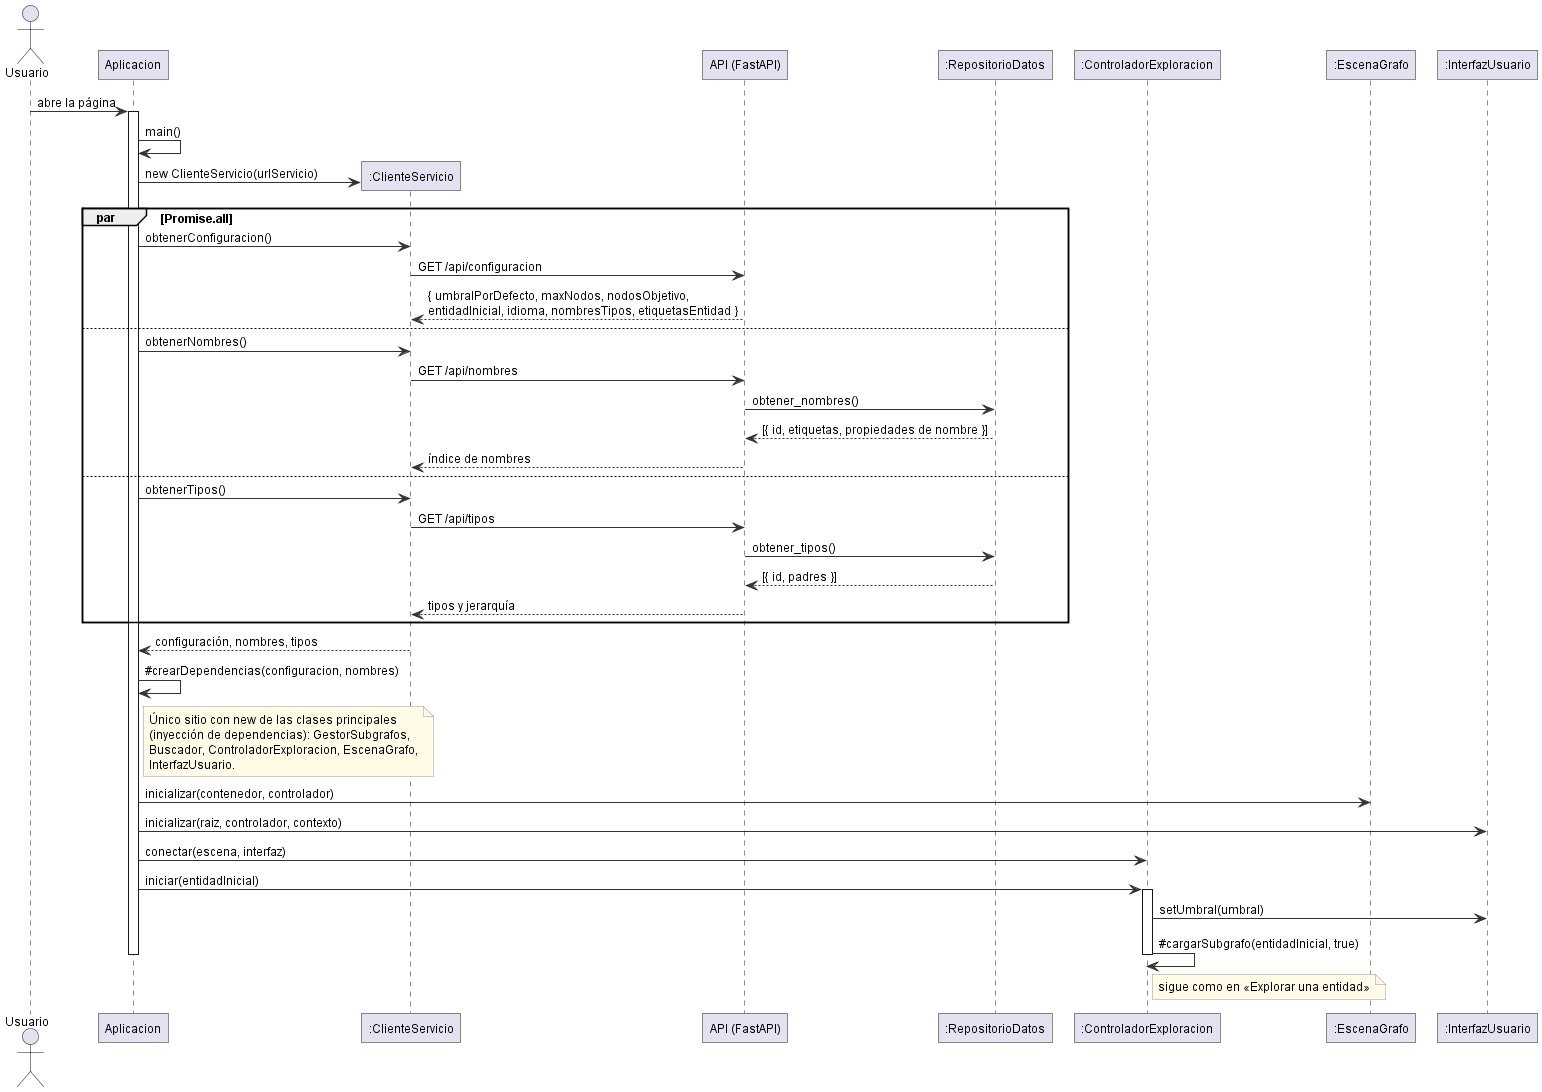
\includegraphics[width=\textwidth]{diagramas/sec_cargar.png}
  \caption{Secuencia de carga de la aplicación.}
  \label{fig:sec-cargar}
\end{figure}

\subsection{Buscar una entidad}

La búsqueda (figura~\ref{fig:sec-buscar}) no genera peticiones: \texttt{PanelBusqueda} espera 150~ms sin pulsaciones y pide sugerencias al controlador, que las obtiene del \texttt{Buscador} sobre el índice en memoria. El diagrama muestra que la vista no habla con el \texttt{Buscador} directamente, sino a través del controlador.

\begin{figure}[htbp]
  \centering
  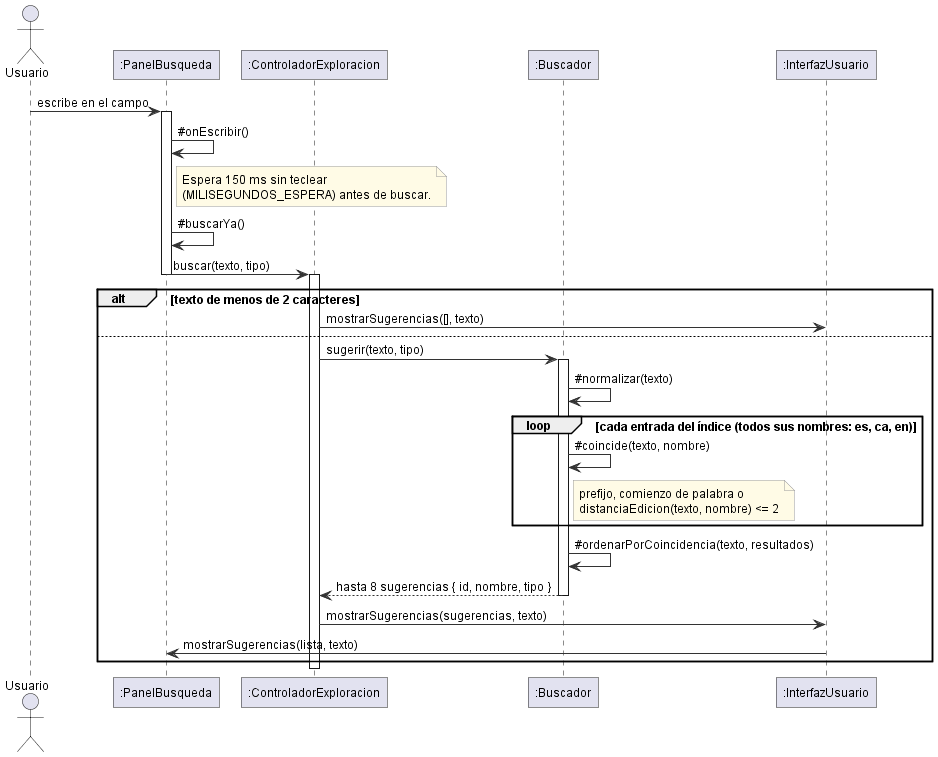
\includegraphics[width=0.9\textwidth]{diagramas/sec_buscar.png}
  \caption{Secuencia de búsqueda de una entidad.}
  \label{fig:sec-buscar}
\end{figure}

\subsection{Explorar una entidad}

Es la operación principal y se divide en dos diagramas. En el navegador (figura~\ref{fig:sec-explorar-cliente}), el controlador pide el subgrafo ajustado a \texttt{GestorSubgrafos}, que solo pide el vecindario si no tiene uno válido guardado; después \texttt{ConstructorSubgrafo} construye el subgrafo y \texttt{EscenaGrafo} lo dibuja. El detalle de la entidad central se pide sin esperar, para que la vista 3D no dependa de él.

\begin{figure}[htbp]
  \centering
  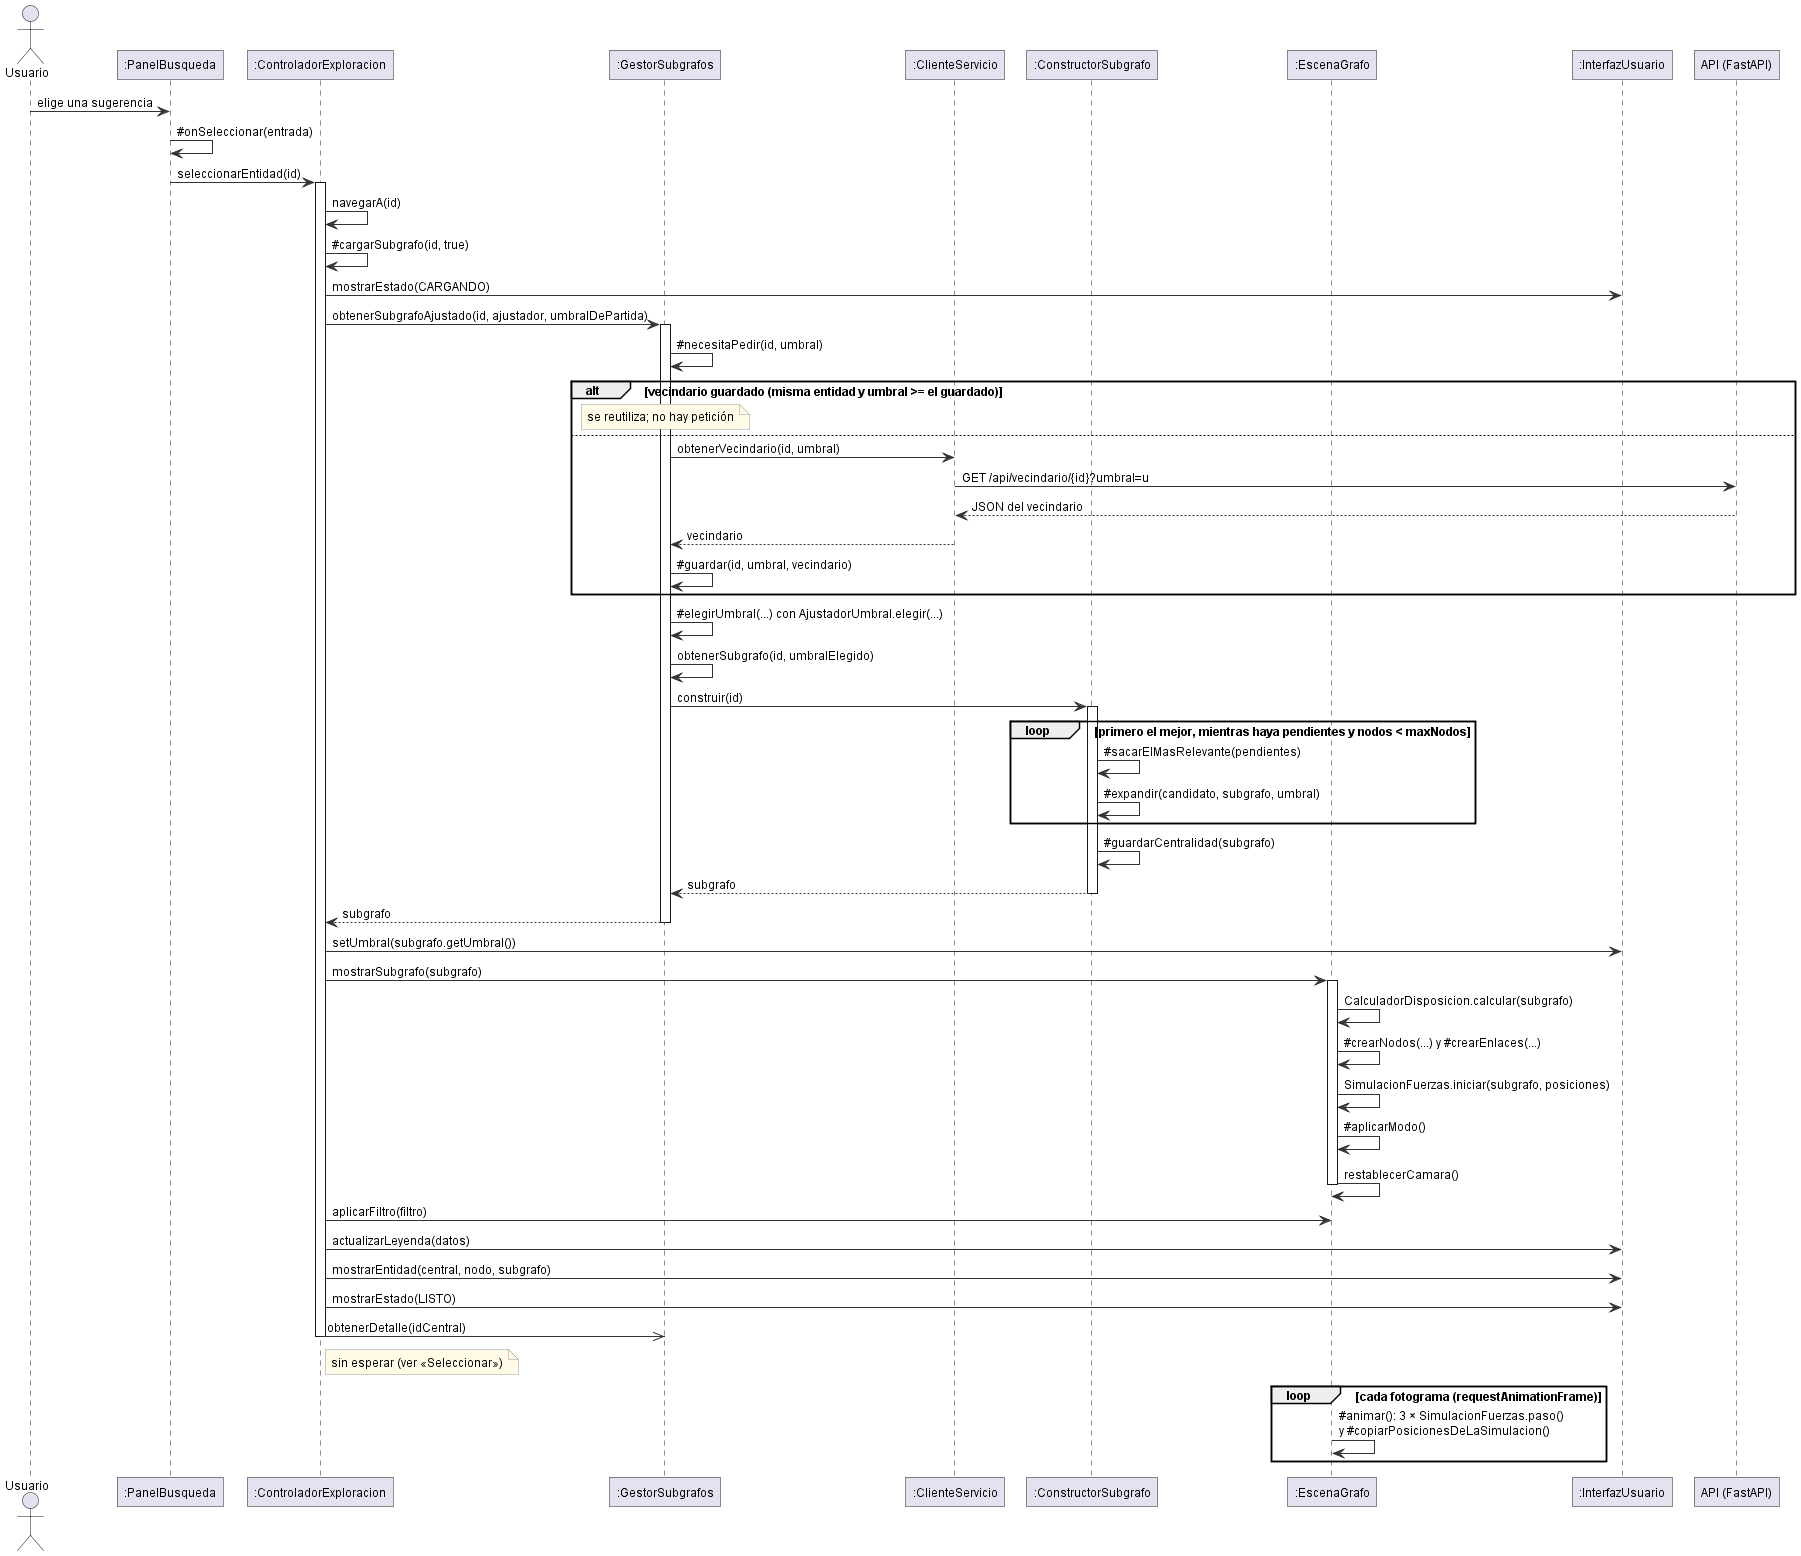
\includegraphics[width=\textwidth]{diagramas/sec_explorar_cliente.png}
  \caption{Secuencia de exploración de una entidad: navegador.}
  \label{fig:sec-explorar-cliente}
\end{figure}

En el servidor (figura~\ref{fig:sec-explorar-servidor}), si la respuesta no está en la caché, \texttt{RepositorioNeo4j} recorre el vecindario. Para cada intermediario, \texttt{AsignadorRelevancia} lee la relevancia guardada y, si falta o es de una versión antigua de los pesos, la calcula con \texttt{RelevanciaPorTipo} y la guarda. El diagrama recoge las dos ramas de la decisión de la sección~\ref{sec:alg-asignacion}.

\begin{figure}[htbp]
  \centering
  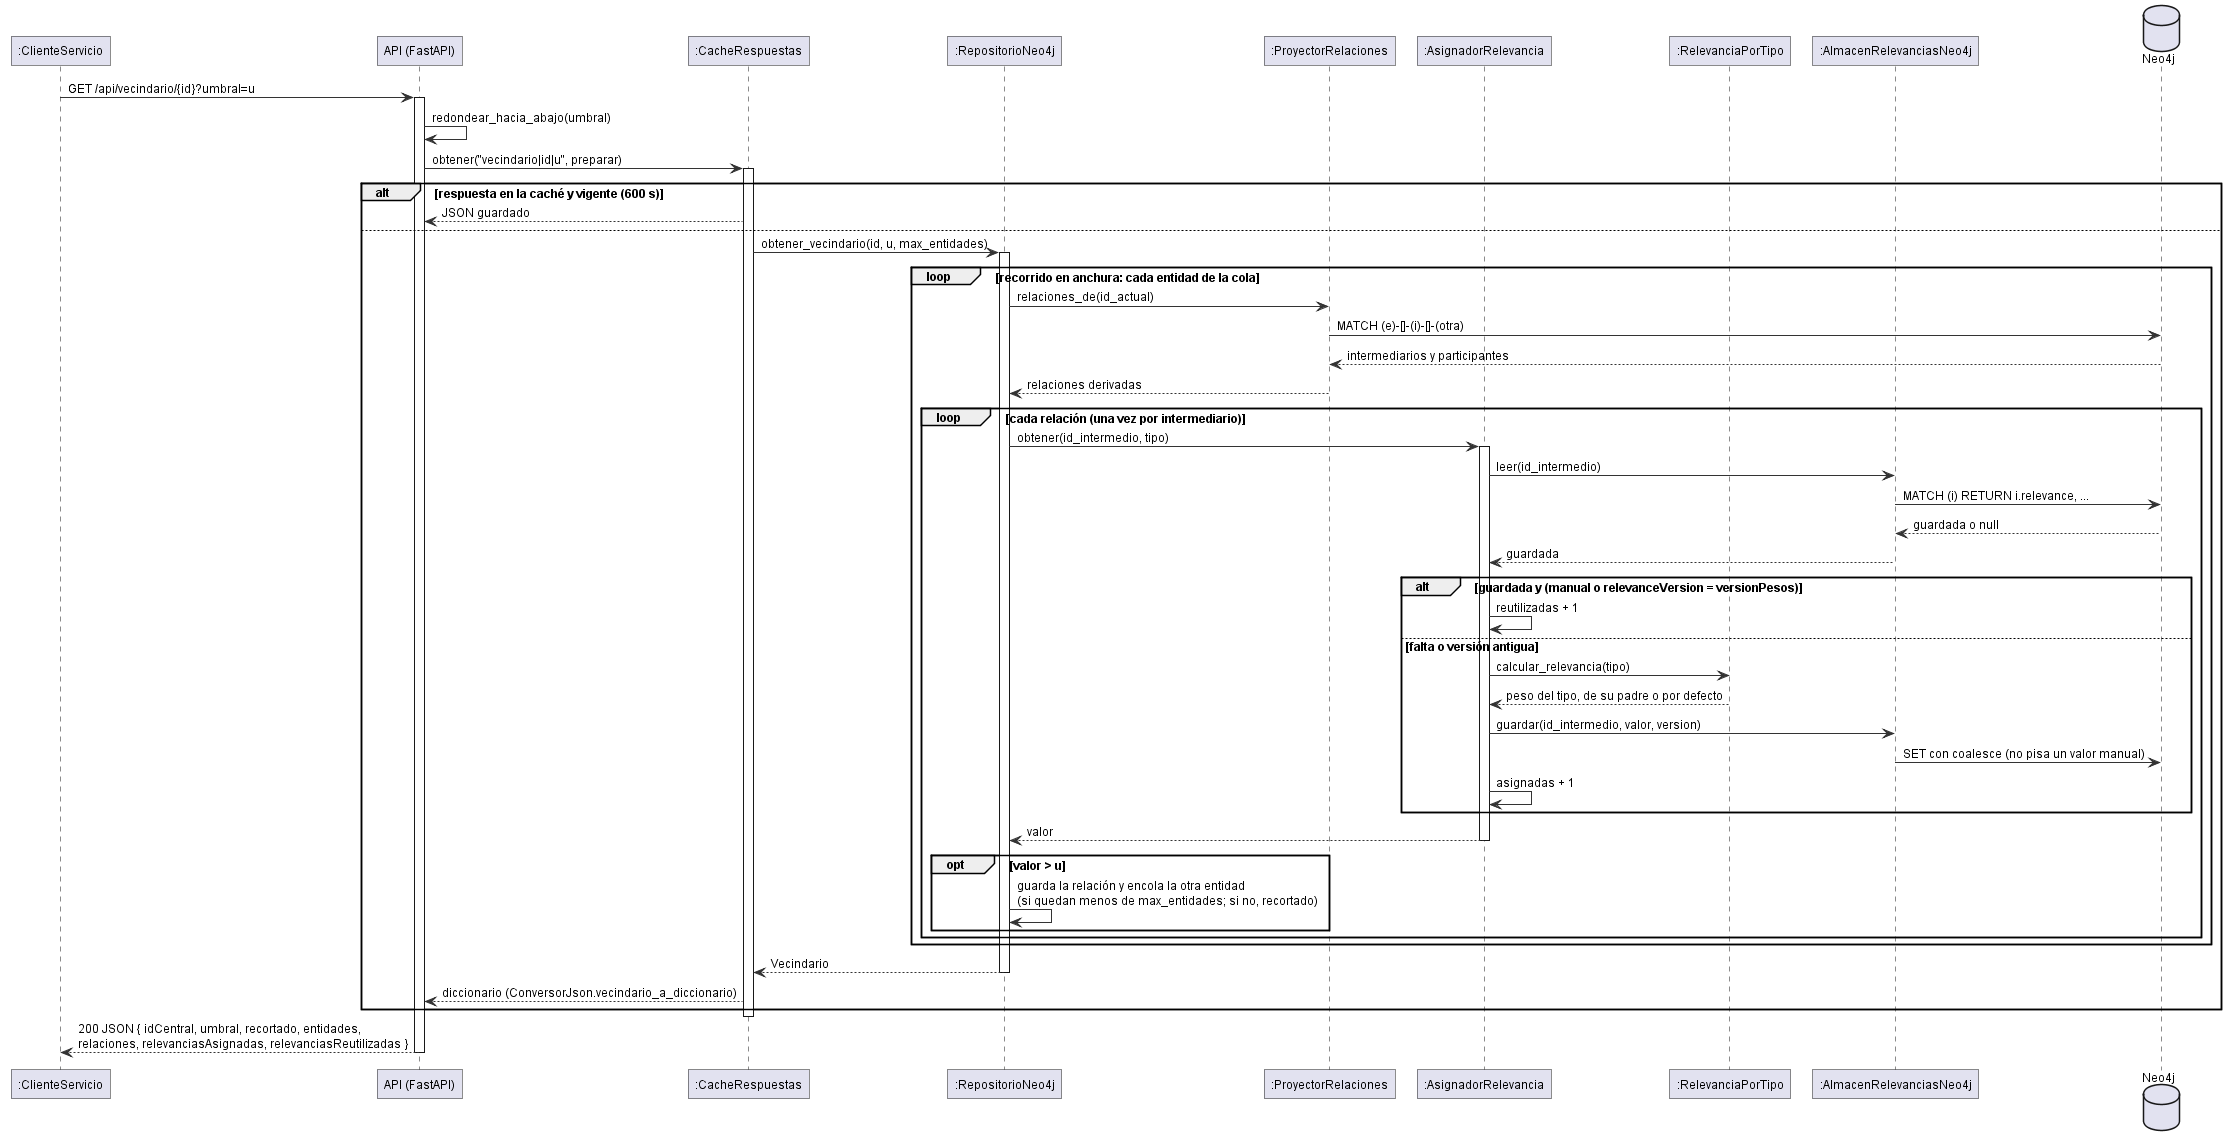
\includegraphics[width=\textwidth]{diagramas/sec_explorar_servidor.png}
  \caption{Secuencia de exploración de una entidad: servidor (incremento~4).}
  \label{fig:sec-explorar-servidor}
\end{figure}

\subsection{Cambiar el umbral}

Al soltar el deslizador (figura~\ref{fig:sec-umbral}), el controlador recalcula el subgrafo de la misma entidad sin ajustar el umbral. El fragmento \texttt{alt} muestra la reutilización: si el umbral sube, el vecindario guardado basta (proposición~\ref{prop:vecindario}) y no hay petición; si baja, se pide un vecindario más amplio.

\begin{figure}[htbp]
  \centering
  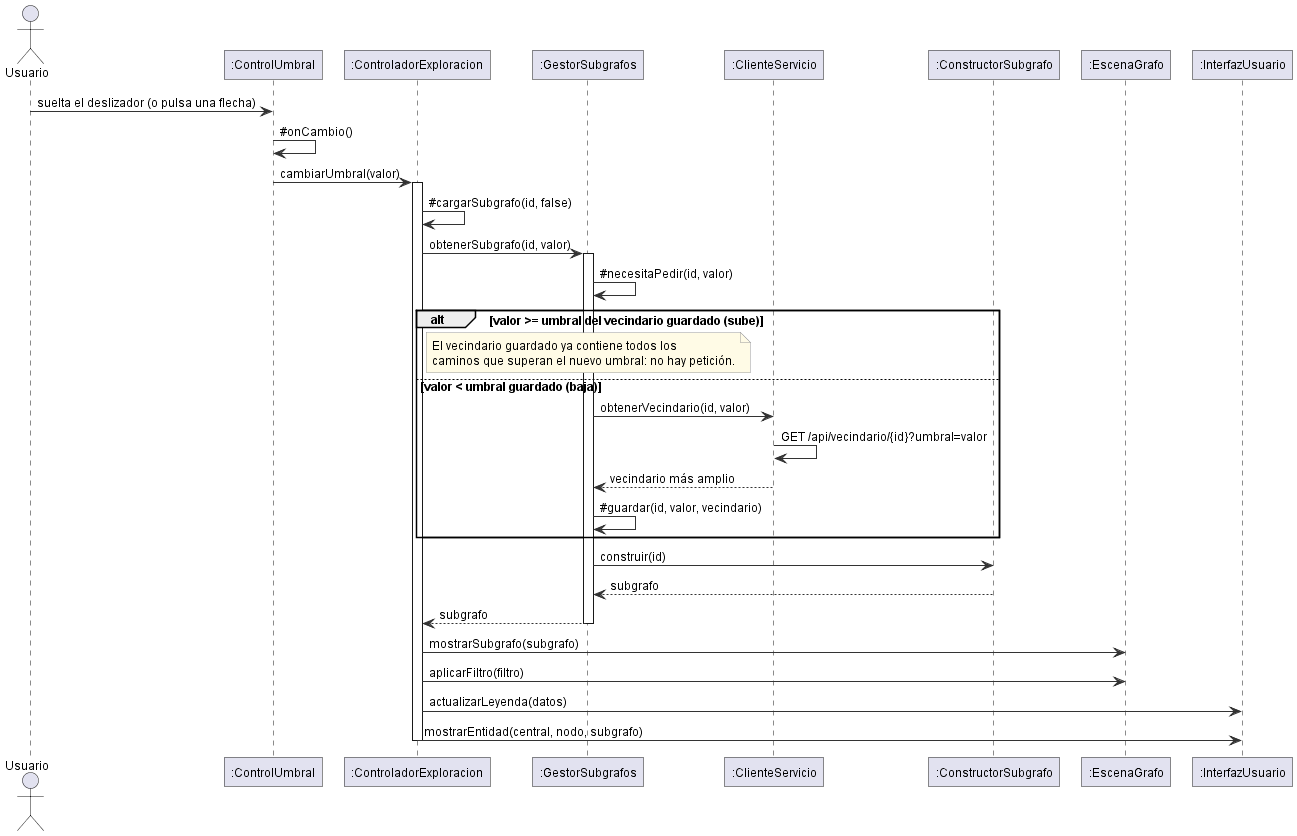
\includegraphics[width=\textwidth]{diagramas/sec_umbral.png}
  \caption{Secuencia de cambio del umbral.}
  \label{fig:sec-umbral}
\end{figure}

\subsection{Seleccionar un nodo o una relación}

\texttt{SelectorInteraccion} distingue un clic de un giro de la cámara por el desplazamiento del puntero (más de 5 píxeles) y localiza el objeto con un rayo (figura~\ref{fig:sec-seleccionar}). Si es un nodo, el controlador lo resalta, muestra su información y pide el detalle sin bloquear; \texttt{GestorSubgrafos} guarda cada detalle para no pedirlo dos veces. Si cuando llega el detalle el usuario ya ha seleccionado otra cosa, se descarta.

\begin{figure}[htbp]
  \centering
  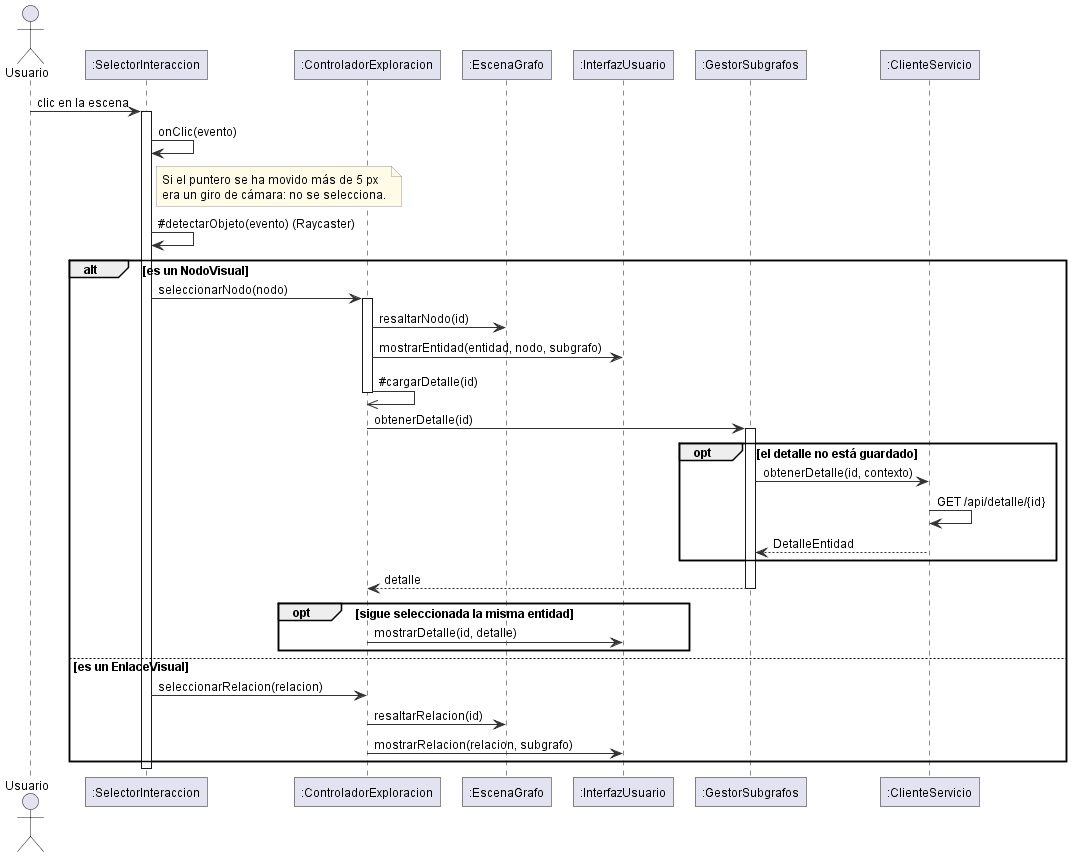
\includegraphics[width=\textwidth]{diagramas/sec_seleccionar.png}
  \caption{Secuencia de selección de un nodo o una relación.}
  \label{fig:sec-seleccionar}
\end{figure}

\subsection{Navegar a un vecino y volver}

Las dos operaciones se agrupan en la figura~\ref{fig:sec-navegar} porque comparten el historial. Navegar (doble clic en un nodo o botón «Explorar su red») apunta la entidad actual en \texttt{HistorialNavegacion} y carga la nueva; volver la recupera sin volver a apuntarla. Las dos reutilizan \texttt{\#cargarSubgrafo}, que numera cada carga para descartar las respuestas que llegan después de una petición más reciente.

\begin{figure}[htbp]
  \centering
  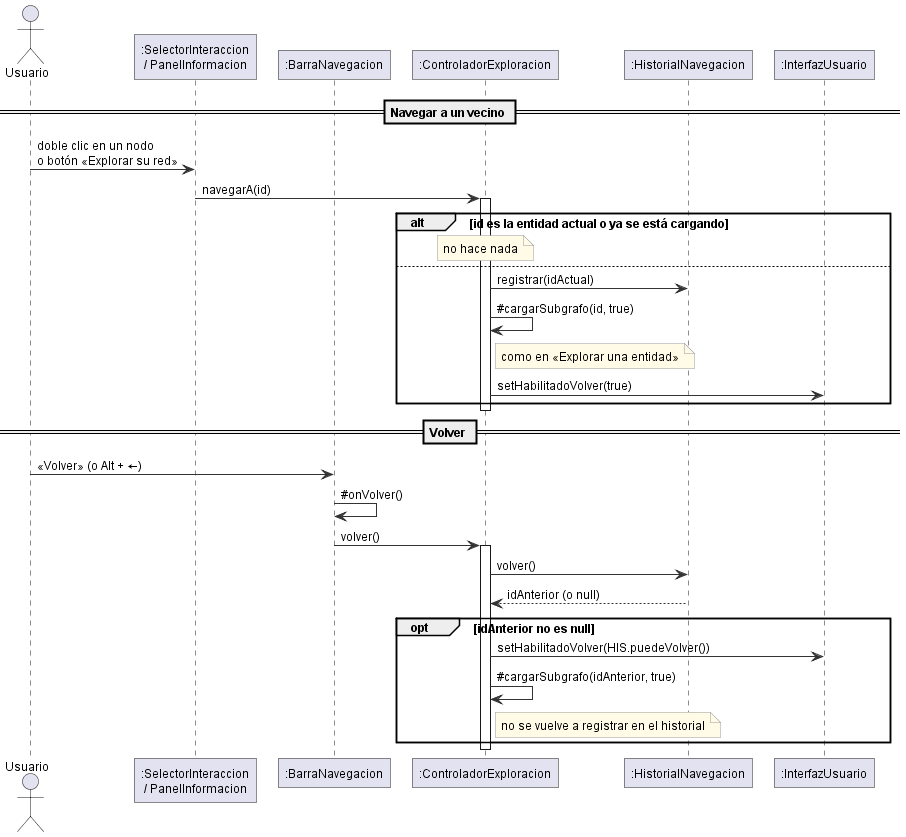
\includegraphics[width=0.9\textwidth]{diagramas/sec_navegar.png}
  \caption{Secuencia de navegación y vuelta atrás.}
  \label{fig:sec-navegar}
\end{figure}

\subsection{Filtrar y cambiar la disposición}

Se agrupan en la figura~\ref{fig:sec-filtrar} las operaciones que solo cambian lo que se ve, sin peticiones ni recálculo del subgrafo: ocultar o mostrar un tipo desde la leyenda, los botones «Todas» y «Ninguna», y el cambio de modo de disposición. En el filtrado, la escena consulta a \texttt{FiltroVisualizacion} si cada objeto es visible; el filtro no conoce la escena. El cambio de disposición recalcula los grupos y reactiva la simulación, de modo que los nodos se desplazan poco a poco a su nueva zona.

\begin{figure}[htbp]
  \centering
  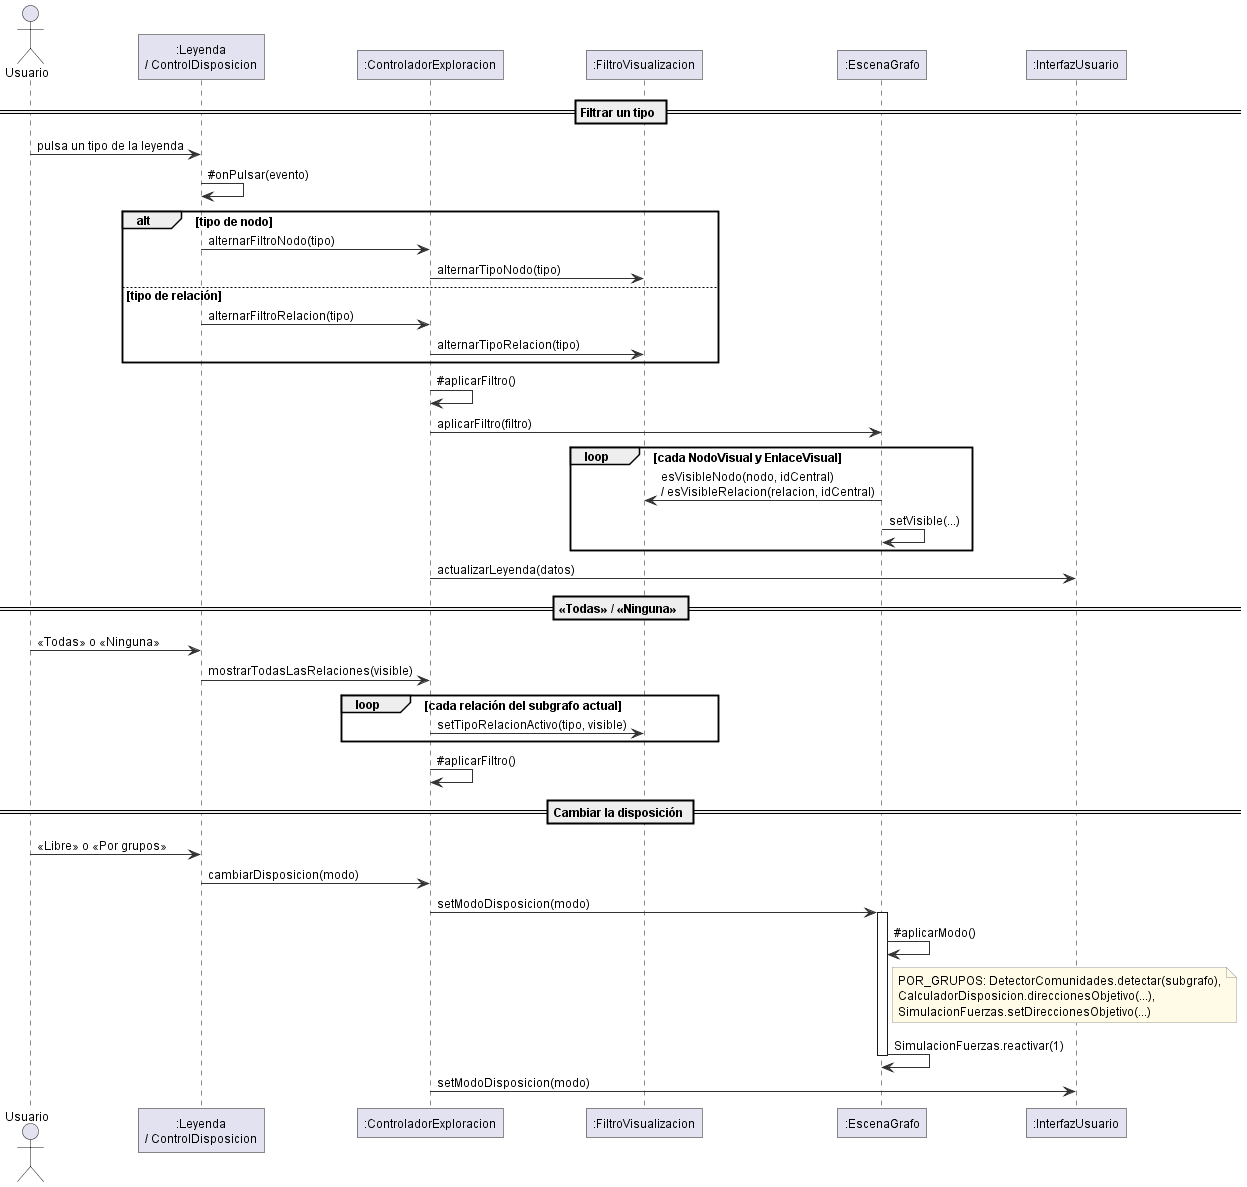
\includegraphics[width=0.9\textwidth]{diagramas/sec_filtrar.png}
  \caption{Secuencia de filtrado y cambio de disposición.}
  \label{fig:sec-filtrar}
\end{figure}

\subsection{Pasar el puntero por encima}

Es la operación más sencilla (figura~\ref{fig:sec-puntero}) y la única que no pasa por el controlador, porque no cambia el estado de la aplicación. Muestra el nombre del nodo, o el tipo y los extremos de la relación, en una etiqueta junto al puntero. El texto se escribe con \texttt{textContent}, para que un nombre procedente de la base de datos nunca se interprete como HTML.

\begin{figure}[htbp]
  \centering
  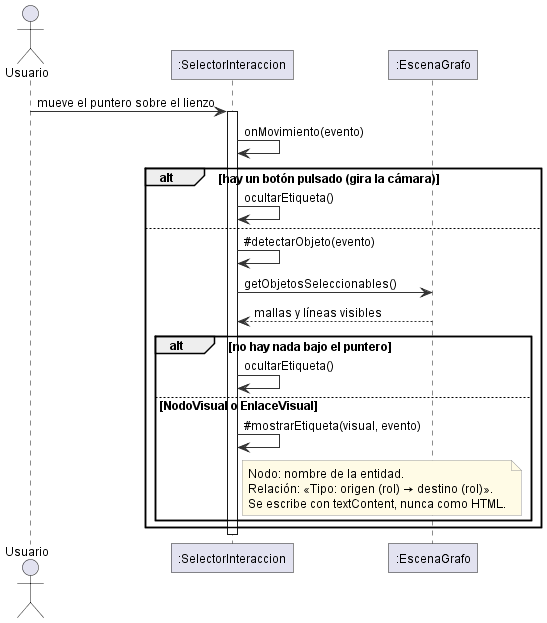
\includegraphics[width=0.75\textwidth]{diagramas/sec_puntero.png}
  \caption{Secuencia de la etiqueta flotante.}
  \label{fig:sec-puntero}
\end{figure}

% ----------------------------------------------------------------------------
\section{Diagrama de paquetes}
\label{sec:paquetes}

La figura~\ref{fig:paquetes} muestra los paquetes del cliente y del servidor con las dependencias que resultan de los \texttt{import} del código, y la frontera HTTP entre los dos.

\begin{figure}[htbp]
  \centering
  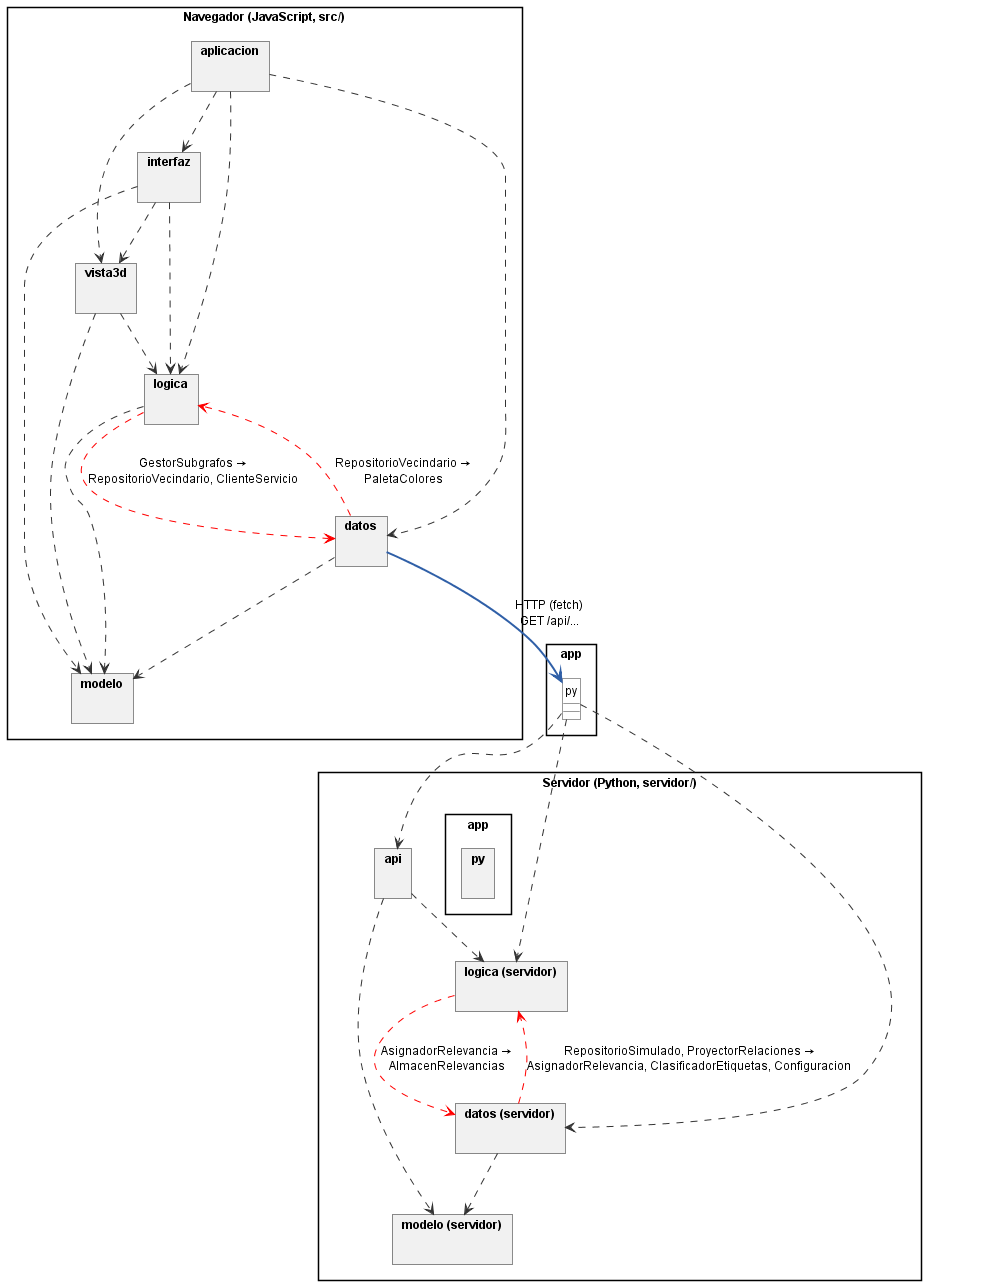
\includegraphics[width=\textwidth]{diagramas/paquetes.png}
  \caption{Diagrama de paquetes. En rojo, las dependencias que forman ciclos.}
  \label{fig:paquetes}
\end{figure}

El cliente sigue una organización en capas: \texttt{aplicacion} crea y conecta todo; \texttt{interfaz} y \texttt{vista3d} son las vistas; \texttt{logica} contiene el controlador y los algoritmos; \texttt{datos} accede al servidor; y \texttt{modelo} contiene las clases del dominio. La regla es que cada capa solo usa las inferiores. \texttt{modelo} no depende de ningún otro paquete, porque todos los demás lo usan: un cambio en la vista o en el acceso a datos no debe afectar a la representación de las entidades.

El análisis de los \texttt{import} muestra dos ciclos, uno en cada lado:
\begin{itemize}
  \item \textbf{Cliente, \texttt{logica} $\leftrightarrow$ \texttt{datos}.} \texttt{GestorSubgrafos} (\texttt{logica}) usa \texttt{ClienteServicio} y \texttt{RepositorioVecindario} (\texttt{datos}), y \texttt{RepositorioVecindario} usa \texttt{PaletaColores} (\texttt{logica}) para dar color a los tipos de relación que descubre.
  \item \textbf{Servidor, \texttt{logica} $\leftrightarrow$ \texttt{datos}.} \texttt{RepositorioSimulado} y \texttt{ProyectorRelaciones} (\texttt{datos}) usan \texttt{AsignadorRelevancia}, \texttt{ClasificadorEtiquetas} y \texttt{Configuracion} (\texttt{logica}), y \texttt{AsignadorRelevancia} usa la interfaz \texttt{AlmacenRelevancias} (\texttt{datos}).
\end{itemize}
En ambos casos el ciclo lo provoca una sola clase mal situada: \texttt{PaletaColores} es una utilidad sin dependencias que podría estar en \texttt{modelo} o en \texttt{vista3d}, y \texttt{AlmacenRelevancias} es una interfaz que define lo que la lógica necesita, por lo que según el principio de inversión de dependencias debería estar en \texttt{logica}. Moverlas eliminaría los dos ciclos sin cambiar el comportamiento. % TODO: decidir si se mueven y actualizar la figura.

En el servidor, \texttt{app} solo depende de \texttt{api}, \texttt{logica} y \texttt{datos}, y \texttt{modelo} no depende de nada. El reparto del trabajo entre los dos lados cumple RNF-05: el servidor solo hace lo que exige acceso a la base de datos (recorrer, derivar y asignar relevancias) y responde con una sola petición por entidad; el cálculo que se repite con cada interacción (subgrafo, centralidad, disposición, búsqueda y filtros) se ejecuta en el navegador de cada usuario.

\subsection{Despliegue}

La figura~\ref{fig:despliegue} muestra el despliegue previsto. Un solo proceso Uvicorn sirve la página ya compilada (\texttt{dist/}, generada con \texttt{npm run build}) y la API, de modo que la página y la API comparten origen y no hace falta configurar CORS. El servidor de aplicación se conecta a Neo4j por el protocolo Bolt con el controlador oficial y lee las credenciales de variables de entorno.

\begin{figure}[htbp]
  \centering
  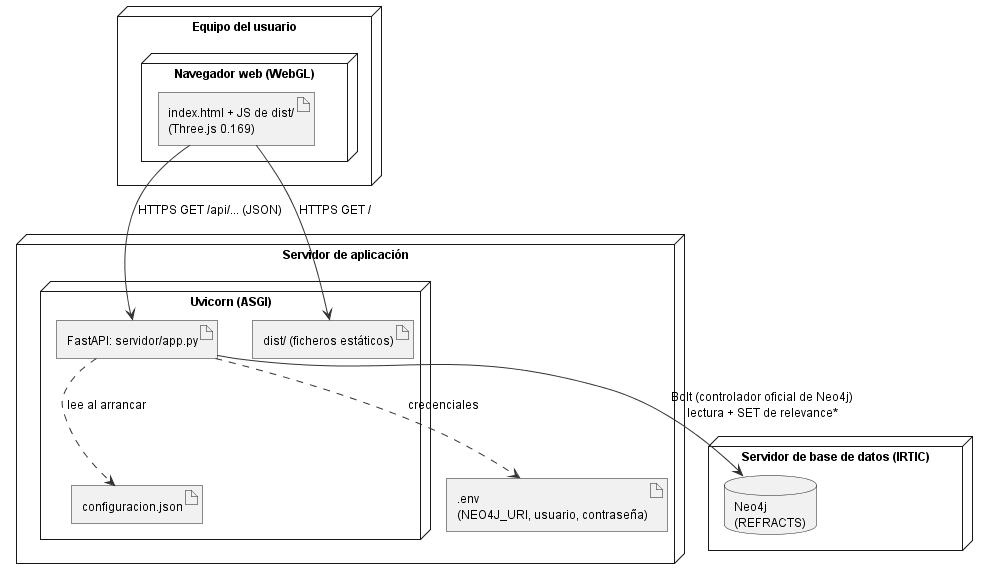
\includegraphics[width=0.85\textwidth]{diagramas/despliegue.png}
  \caption{Diagrama de despliegue.}
  \label{fig:despliegue}
\end{figure}
% TODO: confirmar con el IRTIC dónde se aloja el servidor de aplicación y si Neo4j es accesible desde él.
